\section{Model}

    \begin{frame}{SMODERP1D}
        \begin{columns}
            \begin{column}{0.5\textwidth}
                Posouzení erozní ohroženosti 
                \begin{itemize}
                    \item návrh změny osevních postupů
                    \item umístění ochranných travních pásů
                    \item návrh pásového střídání plodin
                \end{itemize}\vspace{1em}
                Výpočet charakteristik protierozních opatření
                \begin{itemize}
                    \item záchytné a odváděcí prvky
                    \item zasakovací prvky
                    \item prvky měnící podélný sklon
                    \item dráhy soustředěného odtoku
                    \item ochranné nádrže
                \end{itemize}\vspace{1em}
                ke stažení:
                \href{http://storm.fsv.cvut.cz/cinnost-katedry/volne-stazitelne-vysledky/smoderp/smoderp1d/?lang=cz}{storm.fsv.cvut.cz/../smoderp1d/}
            \end{column}
            \begin{column}{0.5\textwidth}
                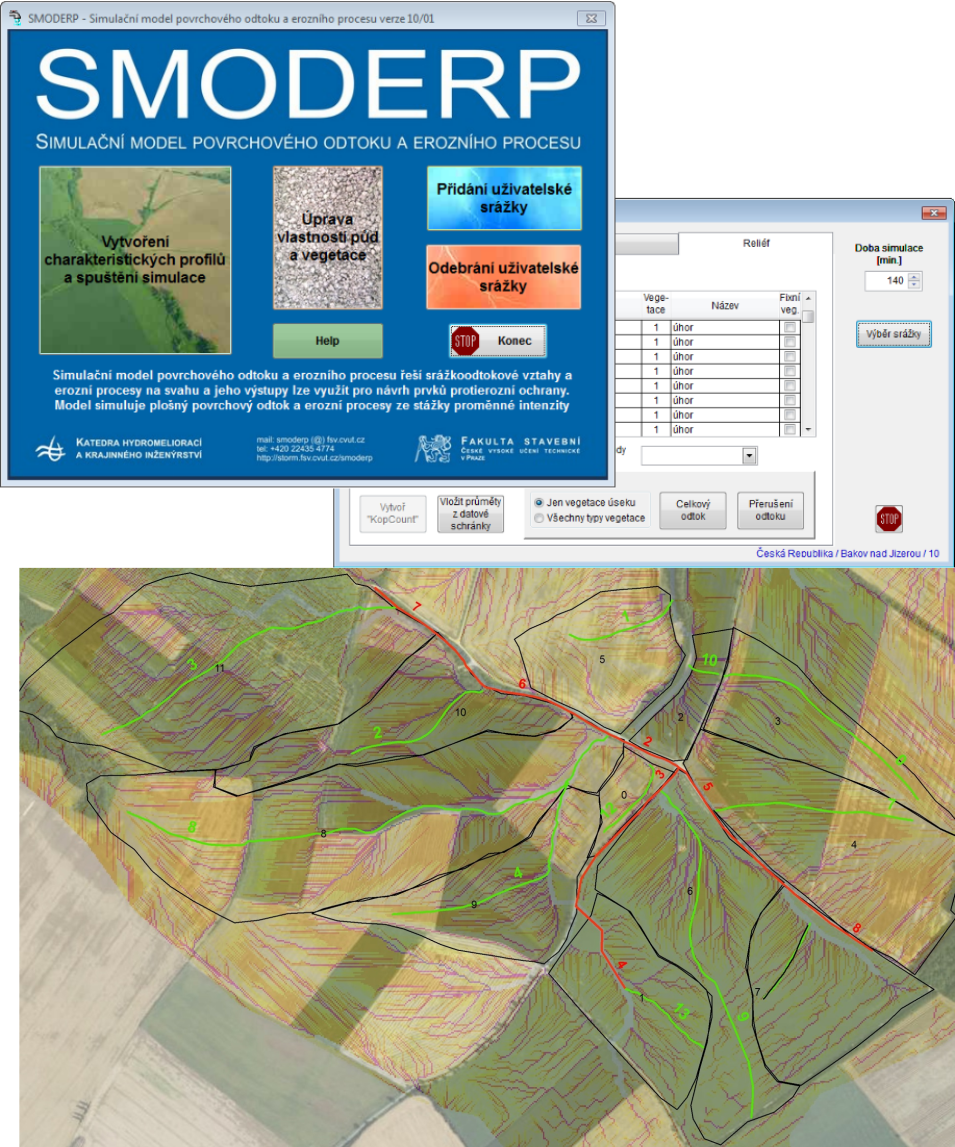
\includegraphics[width=\textwidth]{obr/smode1d.png}
            \end{column}
        \end{columns}
    \end{frame}

    \begin{frame}{SMODERP2D}
    \begin{itemize}\itemsep=1em
            \item Model implementovaný v jazyce {\tt python}
            \item Příprava dat pomocí ArcPy
            \item Oddělený výpočet plošného odtoku, soustředěného odtoku v rýhách
                \begin{itemize}
                    \item dynamické zvětšování rýhy po překročení hraniční hodnoty
                \end{itemize}
            \item Odtok hydrografickou sítí
            \item Dynamický časový krok
            \item Jednosměrný odtokový algoritmus
       \end{itemize}
       \hfill
\includegraphics[height=0.175\textheight]{loga/logsmoderp.png}
    \end{frame}

        \subsection{Použití}

        \begin{frame}
            ArcGIS toolbox:\vspace{-1em}
            \begin{figure}[t!]
            \centering
            \begin{minipage}[t]{.4\textwidth}
              \centering
              \vspace{0pt}
                \begin{figure}
                    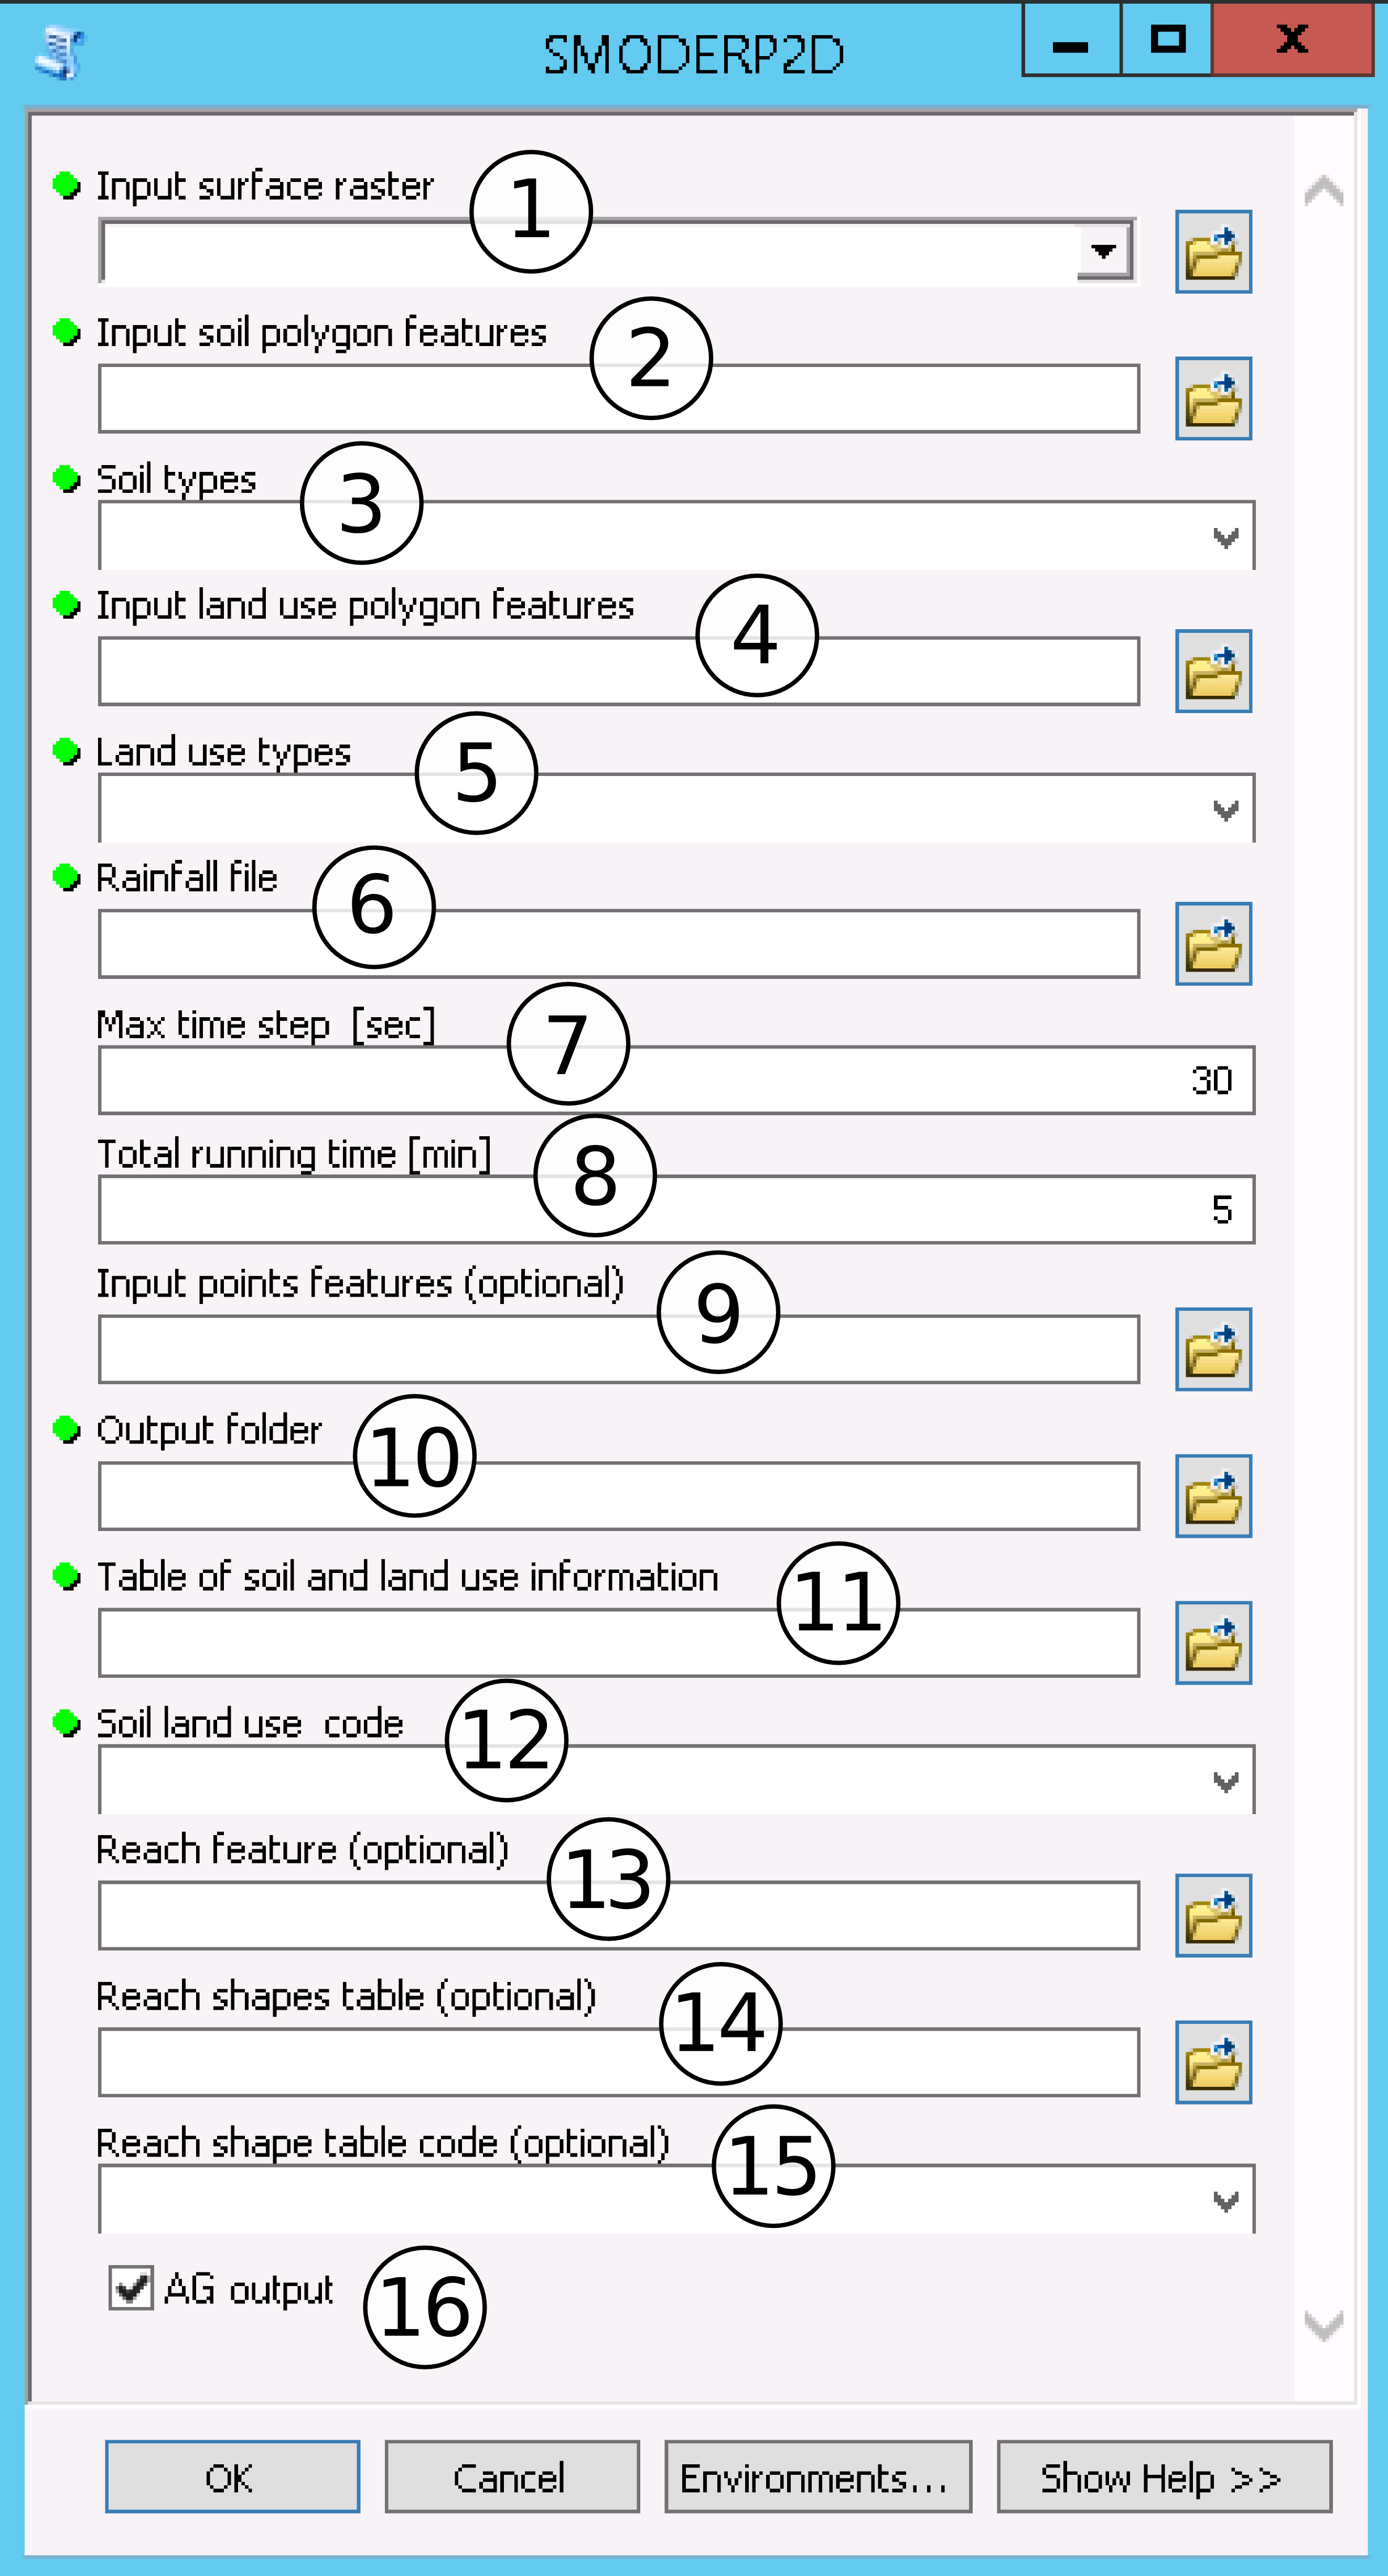
\includegraphics[width=\textwidth]{obr/toolboxpopis4.png}
                \end{figure}
            \end{minipage}\hfill
            \begin{minipage}[t]{.5\textwidth}
              \centering
              \vspace{0pt}
              {\tiny\sffamily
              \begin{tabular}{lp{.5\textwidth}l}
                             & Popis                                       & ArcGIS typ dat     \\
                \hline
            \circled{1}  & Cesta k digitálnímu modlu terénu            &  {\tt Raster layer} \\
            \circled{2}  & Cesta k vektorové vrstvě rozložení typu půd &  {\tt Shapefile} \\
            \circled{3}  & Název pole s id typů půd &  {\tt Field} \\
            \circled{4}  & Cesta k vektorové vrstvě využití území &  {\tt Shapefile} \\
            \circled{5}  & Název pole s id využití území &  {\tt Field} \\
            \circled{6}  & Cesta k souboru se srážkovými daty &  {\tt Text file} \\
            \circled{7}  & Maximální časový krok &  {\tt Double} \\
            \circled{8}  & Konečný čas výpočtu &  {\tt Double} \\
            \circled{9}  & Vrstva bodů pro výpis hydrogramů &  {\tt Shapefile} \\
            \circled{10} & Výstupní adresář &  {\tt Folder} \\
            \circled{11} & Tabulka s parametry modelu &  {\tt Table} \\
            \circled{12} & Označení pole v tabulce \circled{11} &  {\tt Field} \\
            \circled{13} & Cesta k vrstvě linií hydrografické sítě &  {\tt Feature Class} \\
            \circled{14} & Cesta k tabulce s geometrií úseků hydrografické sítě &  {\tt Table} \\
            \circled{15} & Název společného pole pro spojení \circled{13} a \circled{14} &  {\tt Field} \\
            \circled{16} & Volba formy výstupních souborů &  {\tt Boolean} \\
              \end{tabular}
              }
            \end{minipage}
            %\caption{ArcGIS {\tt toolbox} a vysvětlenými parametry}
            \label{fig:toolbox}
          \end{figure}

        \end{frame}

        \begin{frame}
            Testovací data v ArcGIS\vspace{1em}
            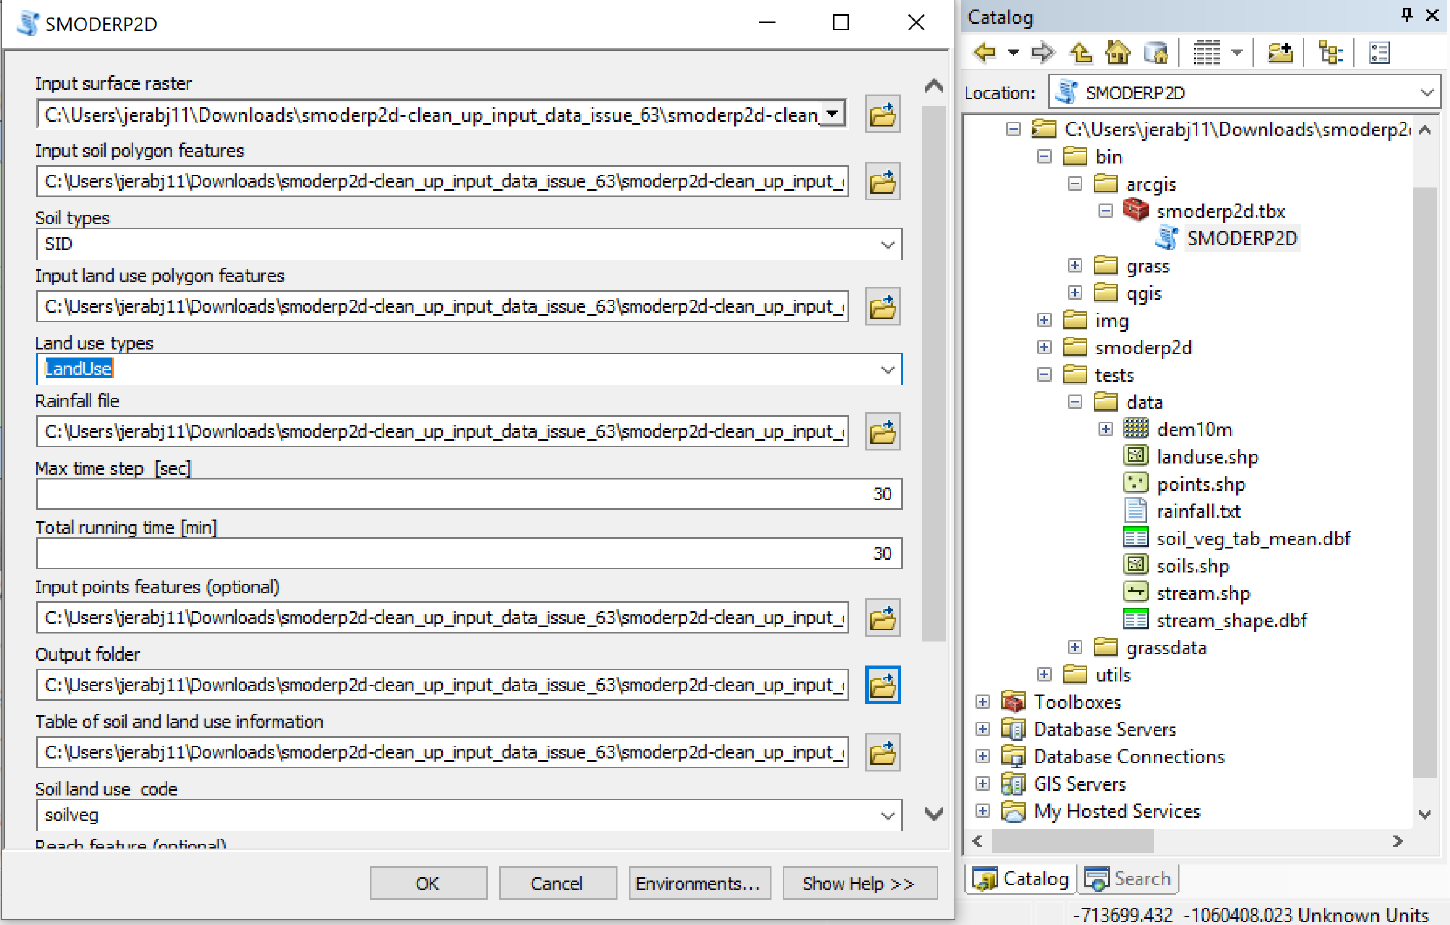
\includegraphics[width=0.95\textwidth]{obr/arcmap01.png}
        \end{frame}

        \begin{frame}\hypertarget{fig}{}
        \Wider[4em]{
            Ukázka přípravy dat v ArcGIS\vspace{1em}: půdní typ a využití území 
            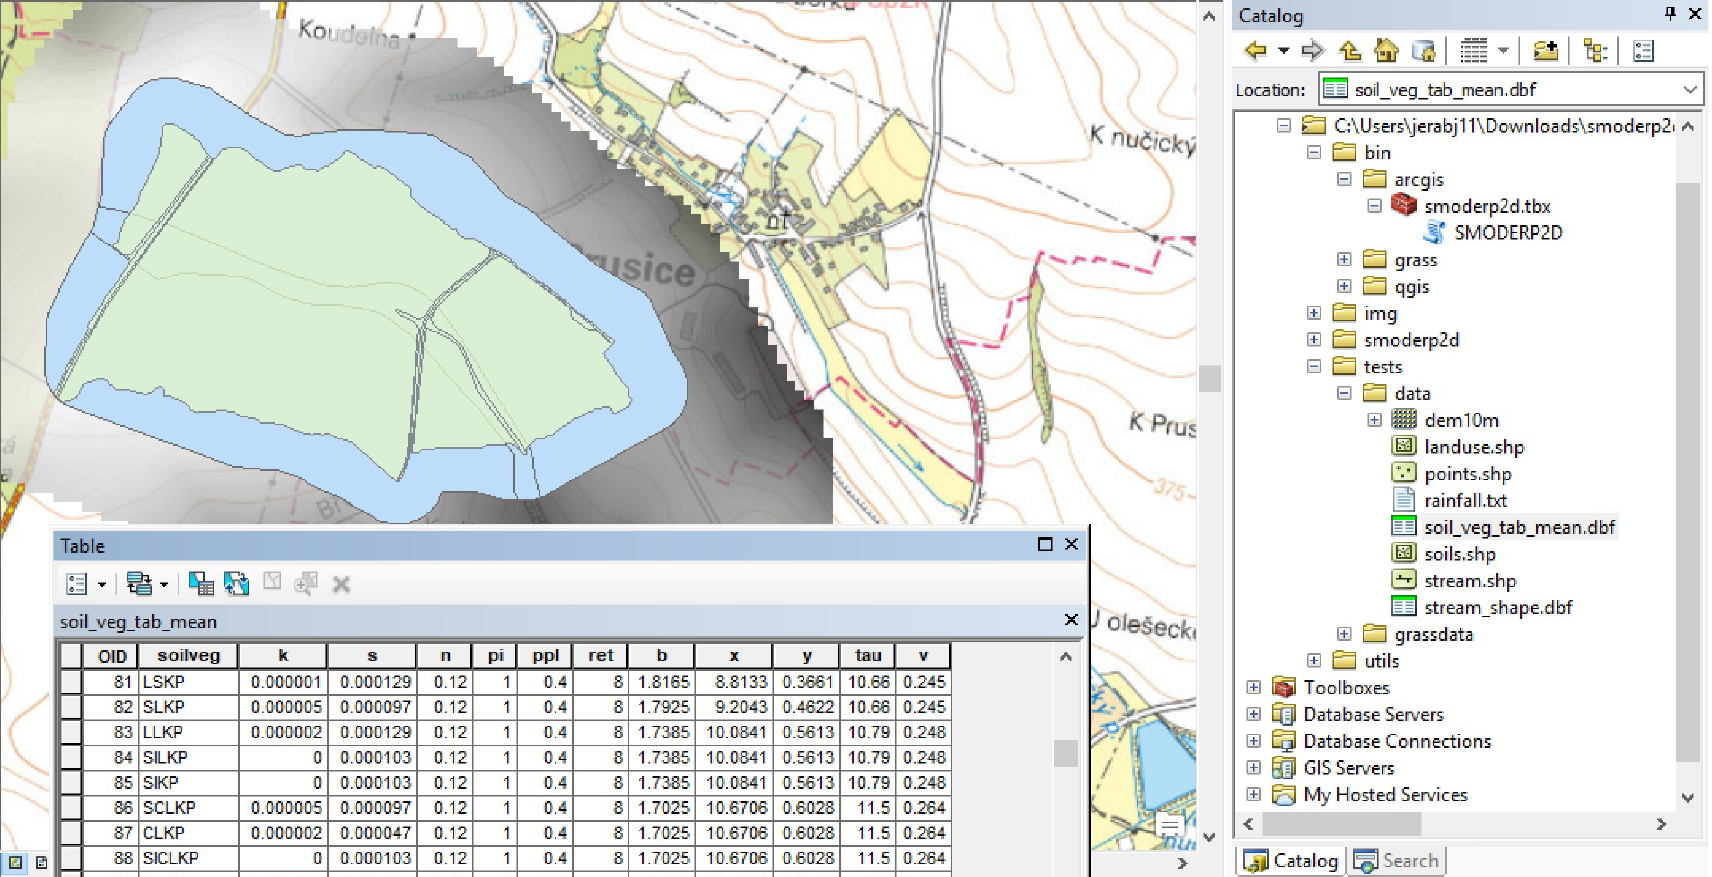
\includegraphics[width=\textwidth]{obr/arcmap02.png}
            Popis sloupečku v atributové tabulce~\ref{tab:soilveg} za konci prezentace.
        }
        \end{frame}
        \begin{frame}
        \Wider[4em]{
            Ukázka přípravy dat v ArcGIS\vspace{1em}: hydrografická síť
            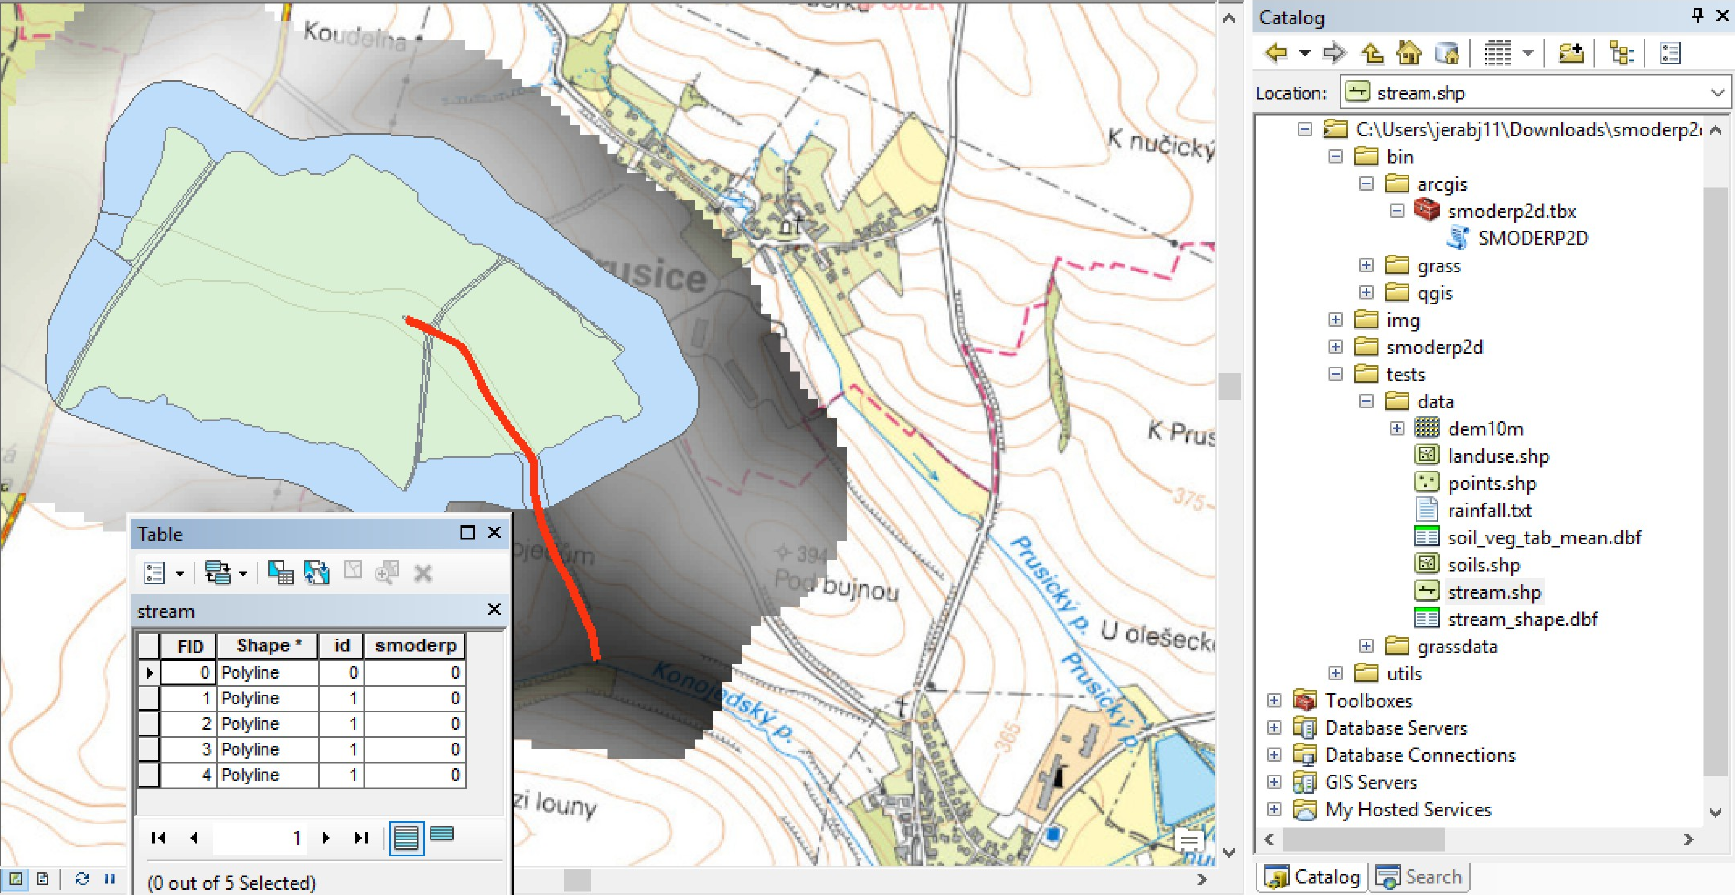
\includegraphics[width=\textwidth]{obr/arcmap03.png}
        }
        \end{frame}
        \begin{frame}
        \Wider[4em]{
            Ukázka přípravy dat v ArcGIS\vspace{1em}: parametry úseků hydrografické sítě
            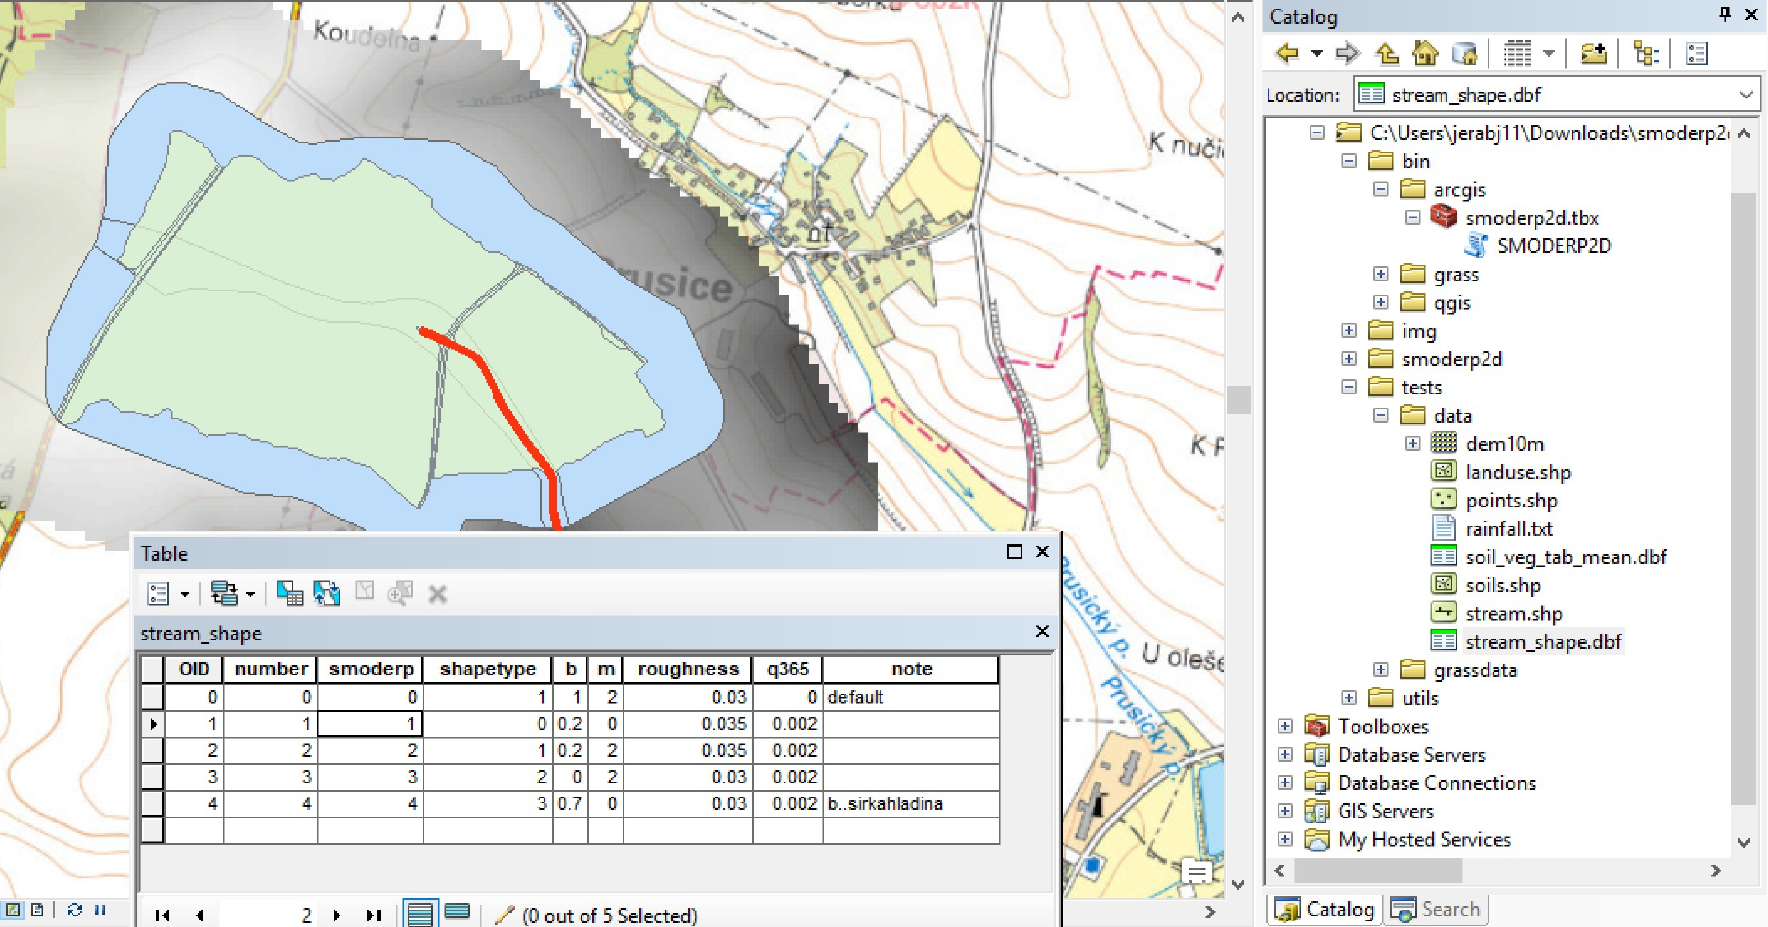
\includegraphics[width=\textwidth]{obr/arcmap04.png}
        }
        \end{frame}
        \begin{frame}
        \Wider[4em]{
            Ukázka přípravy dat v ArcGIS\vspace{1em}: body na výpis výsledků
            \begin{center}
            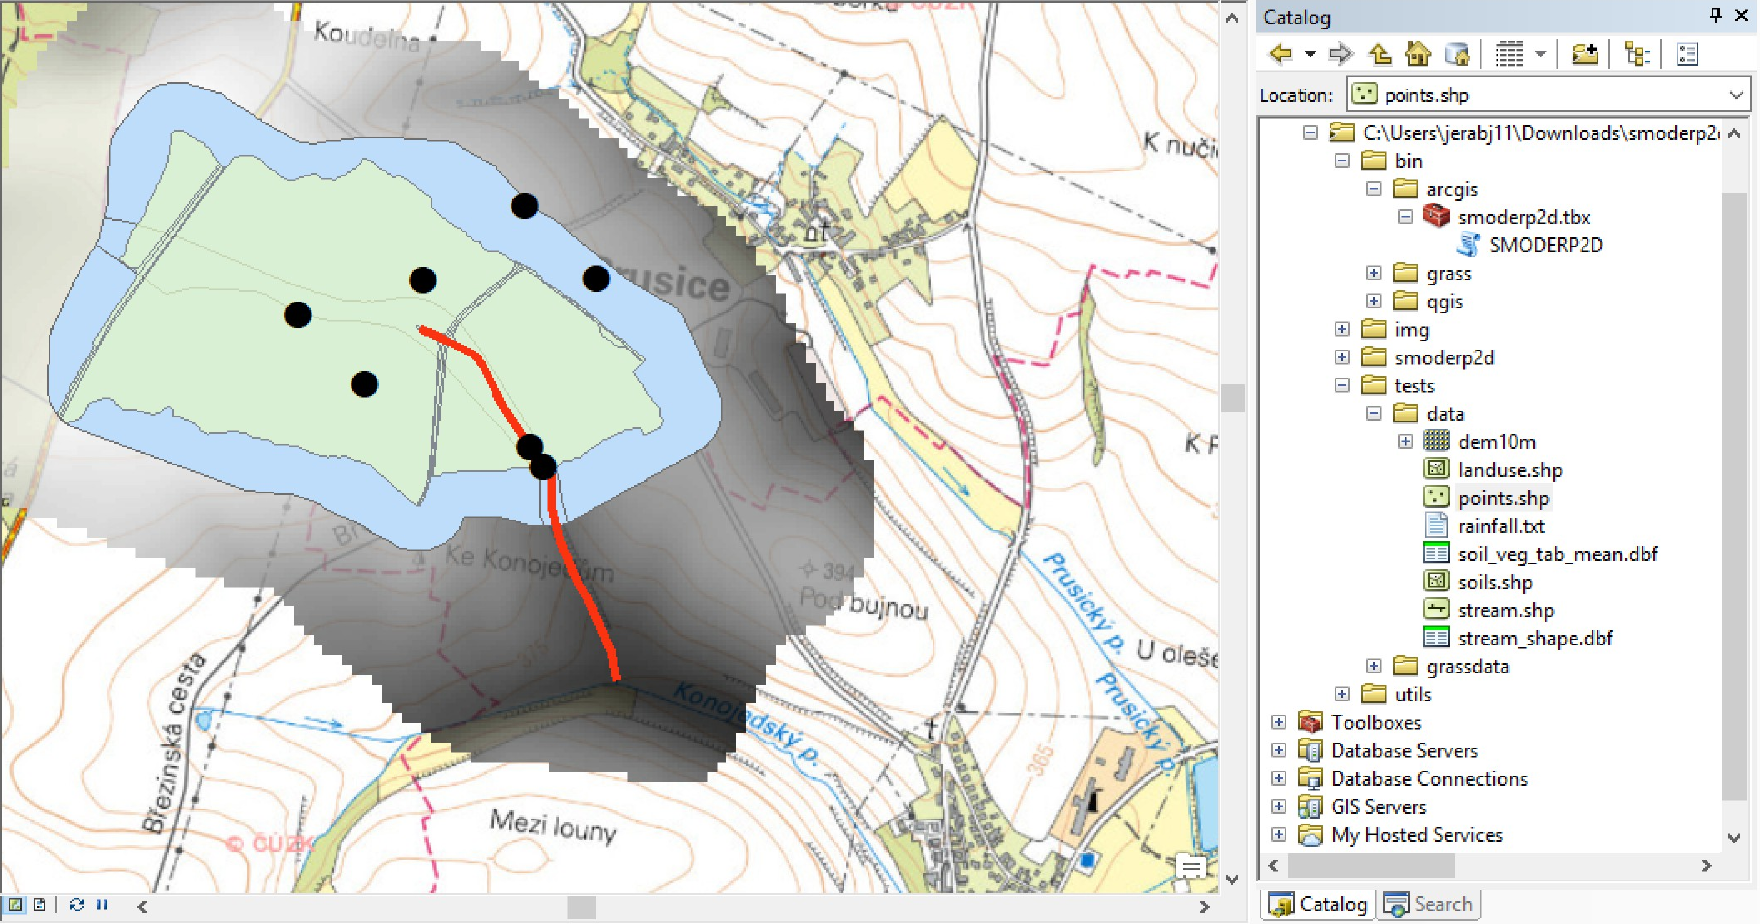
\includegraphics[width=\textwidth]{obr/arcmap05.png}
            \end{center}
        }
        \end{frame}


        \begin{frame}[plain]
            Ukázka výsledků reakce povodí na 40 minut 120 mm/hod srážky
            \begin{adjustwidth}{-3em}{-2em}
                    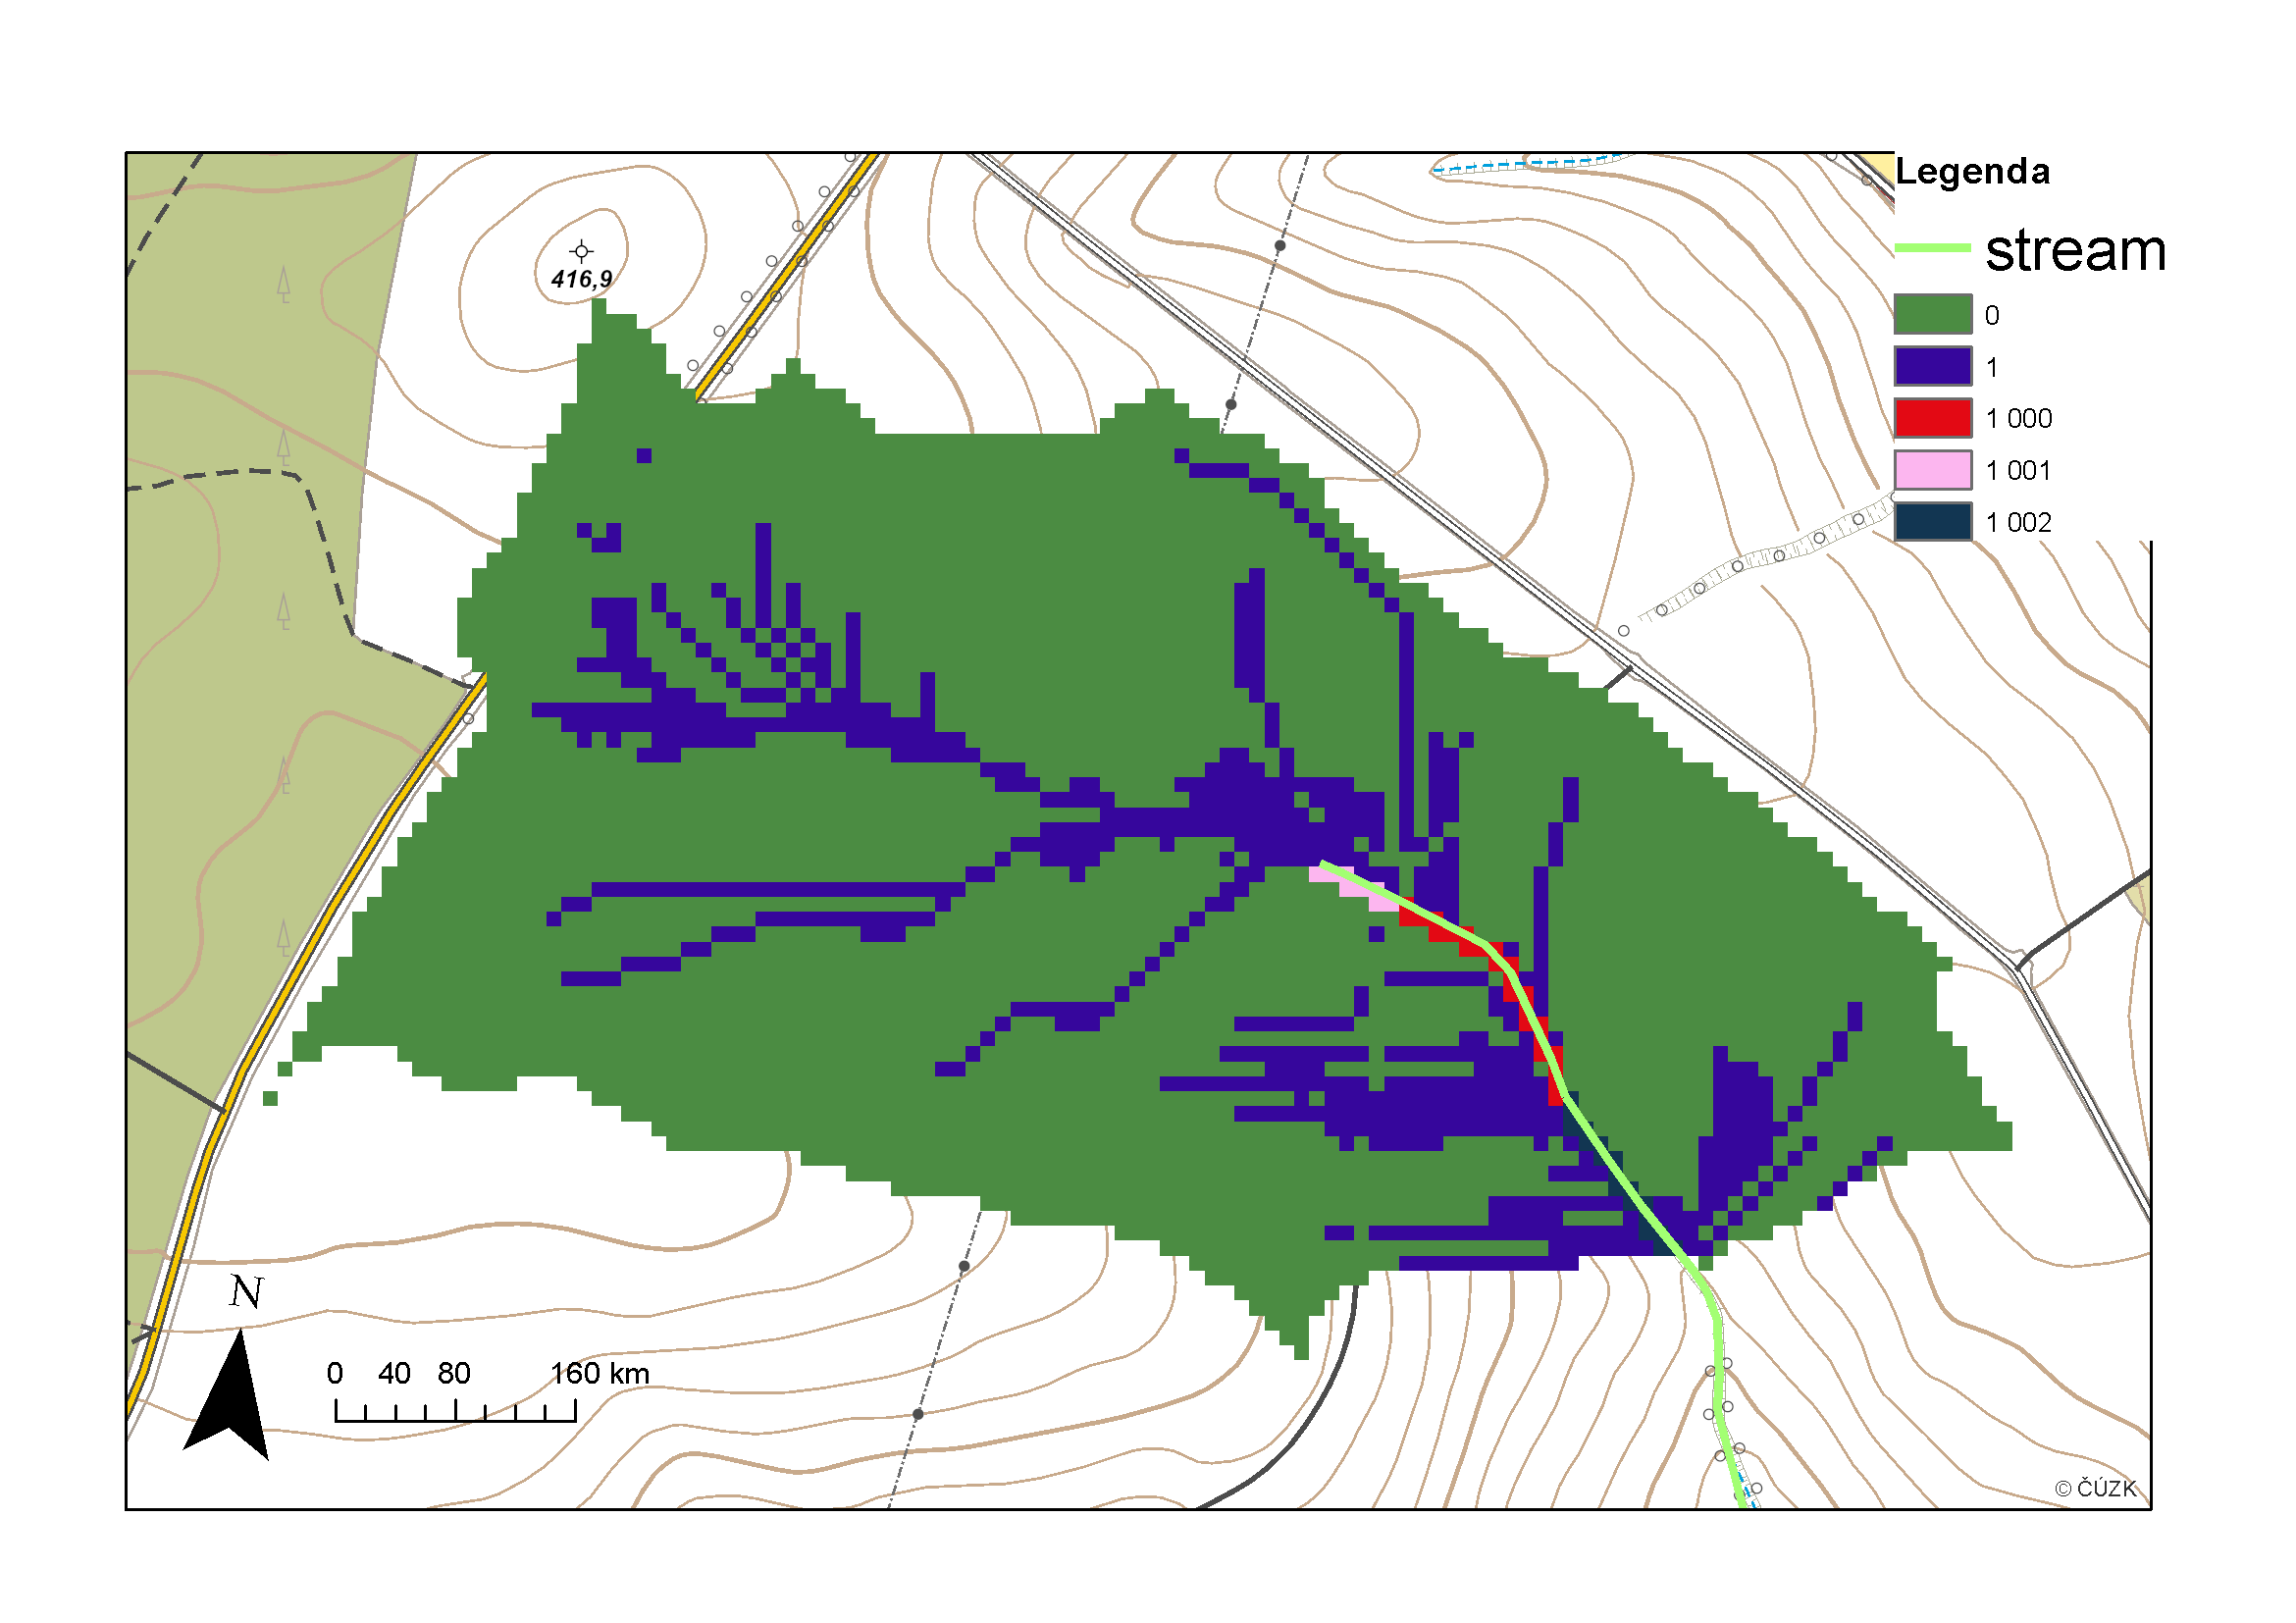
\includegraphics[width=0.55\textwidth]{obr/fstate.png}
                    %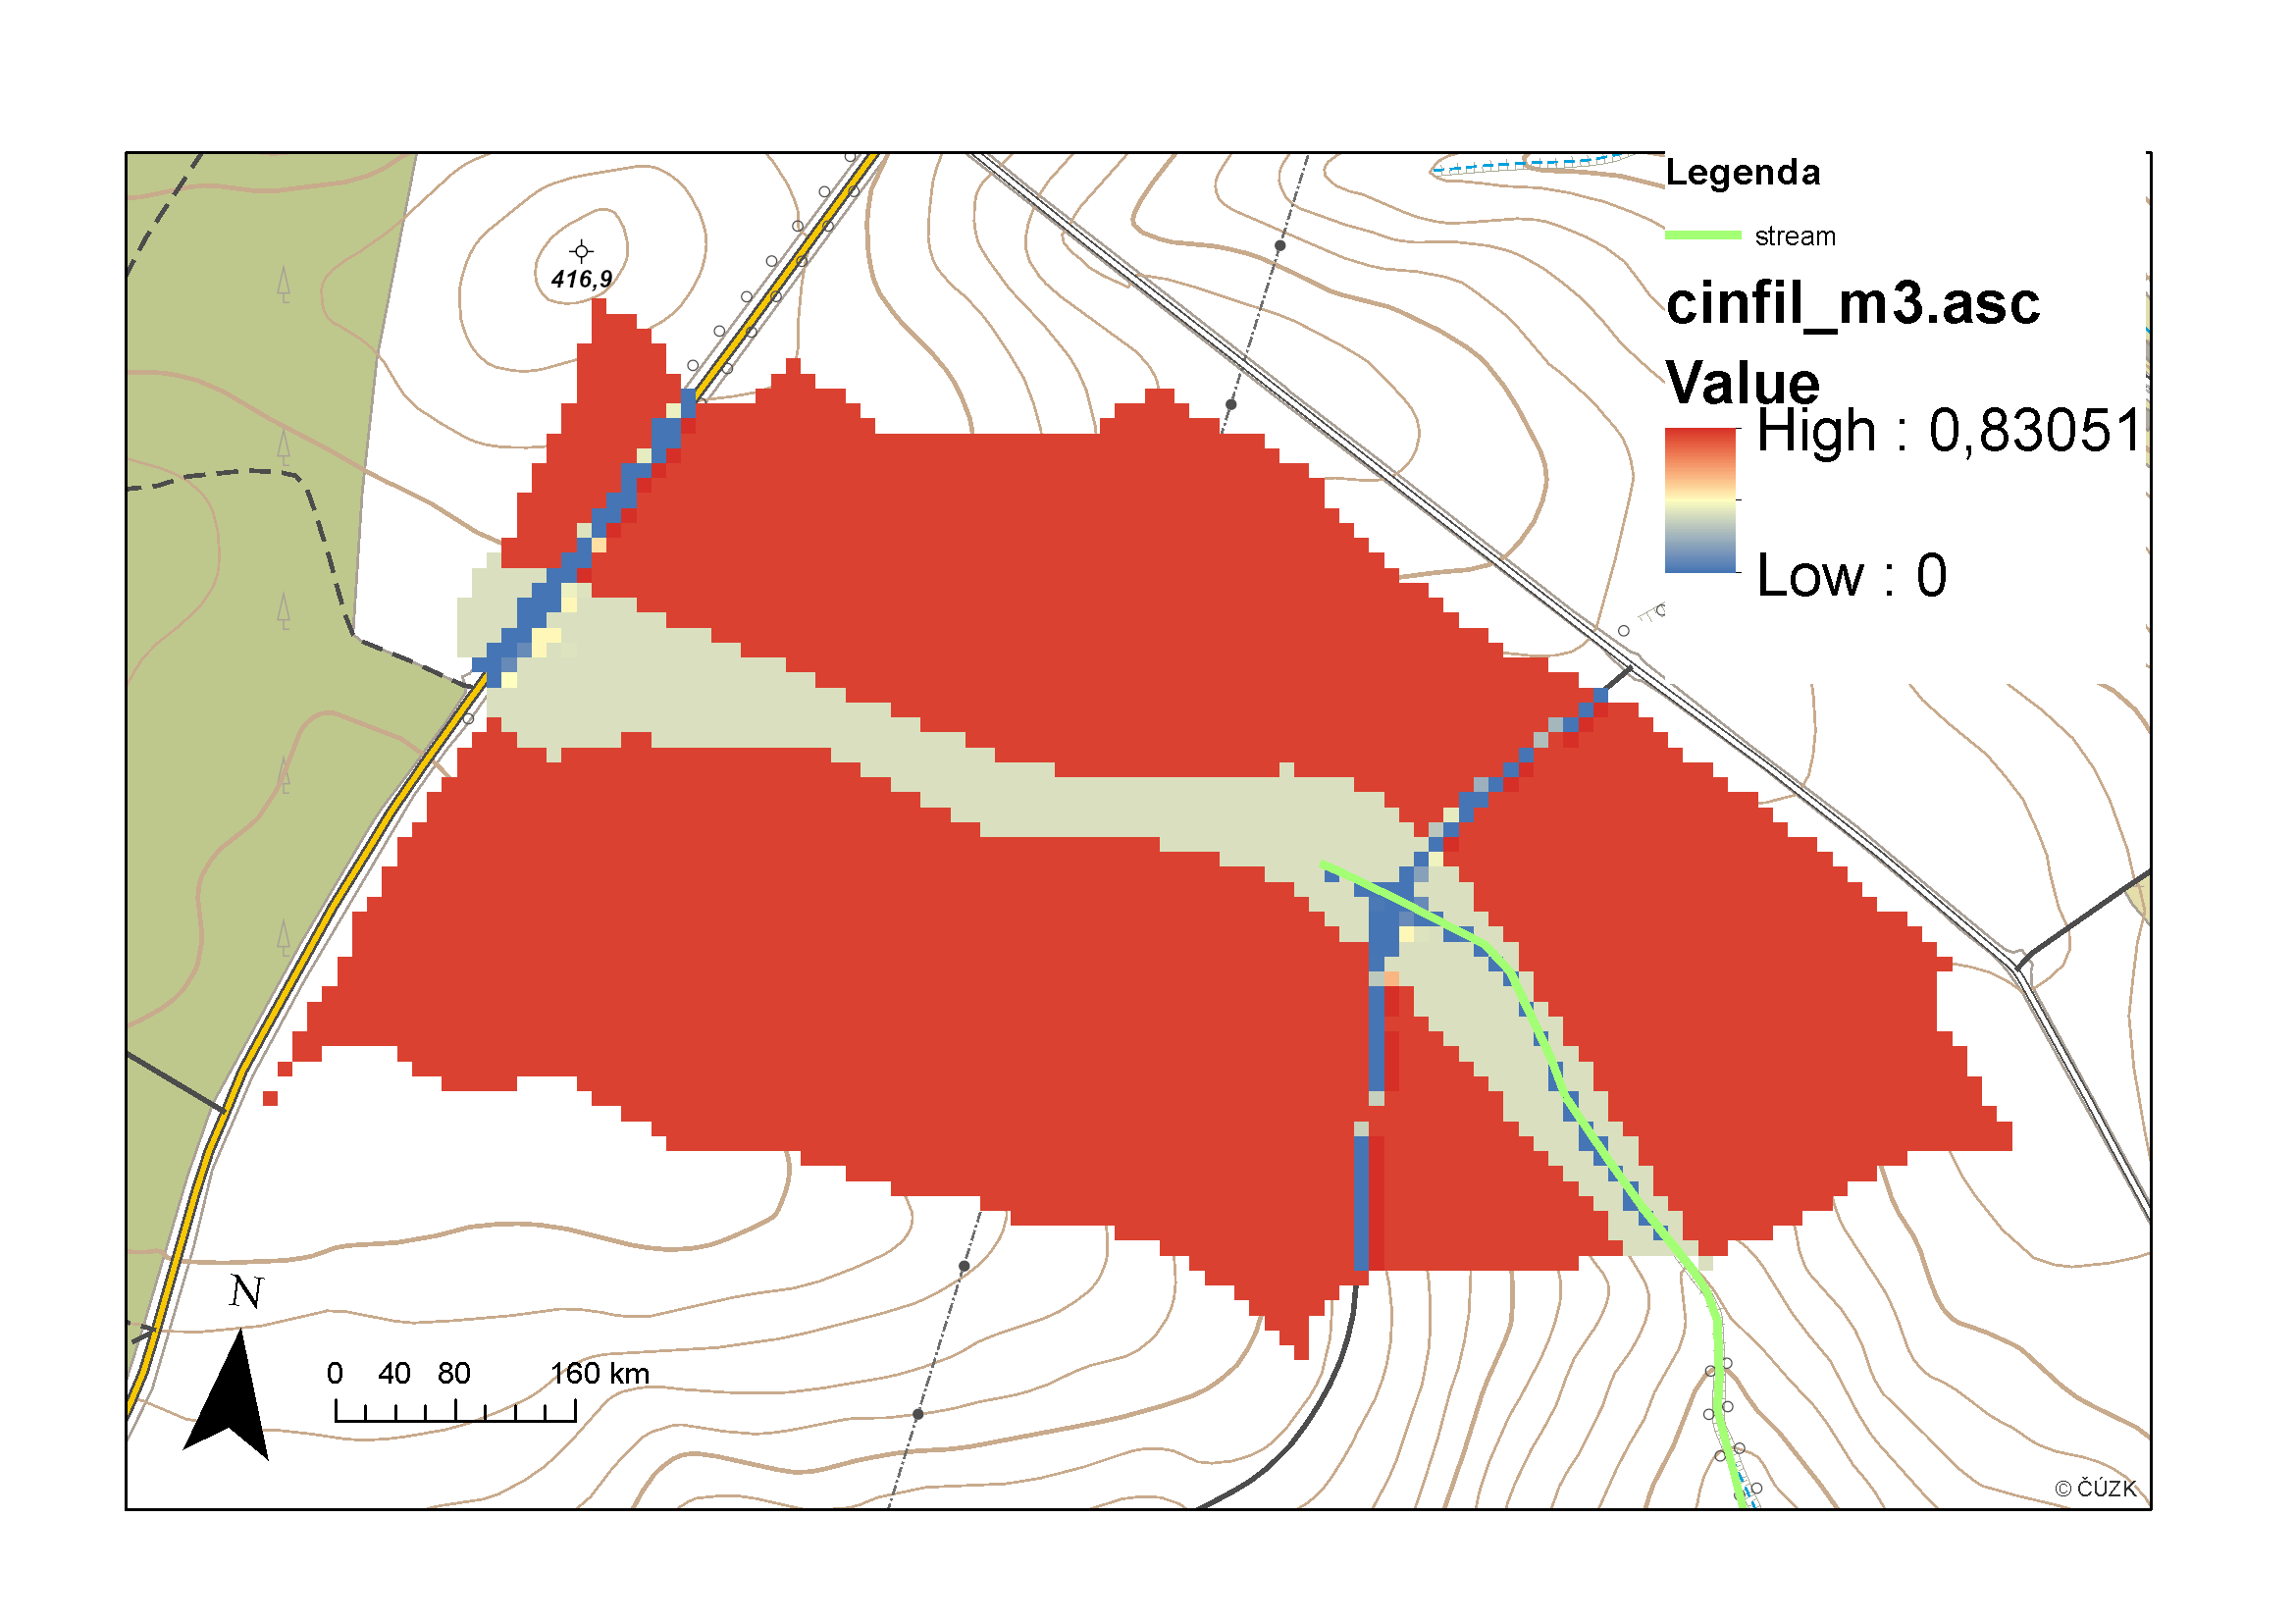
\includegraphics[width=0.55\textwidth]{obr/infiltr.png}\\
                    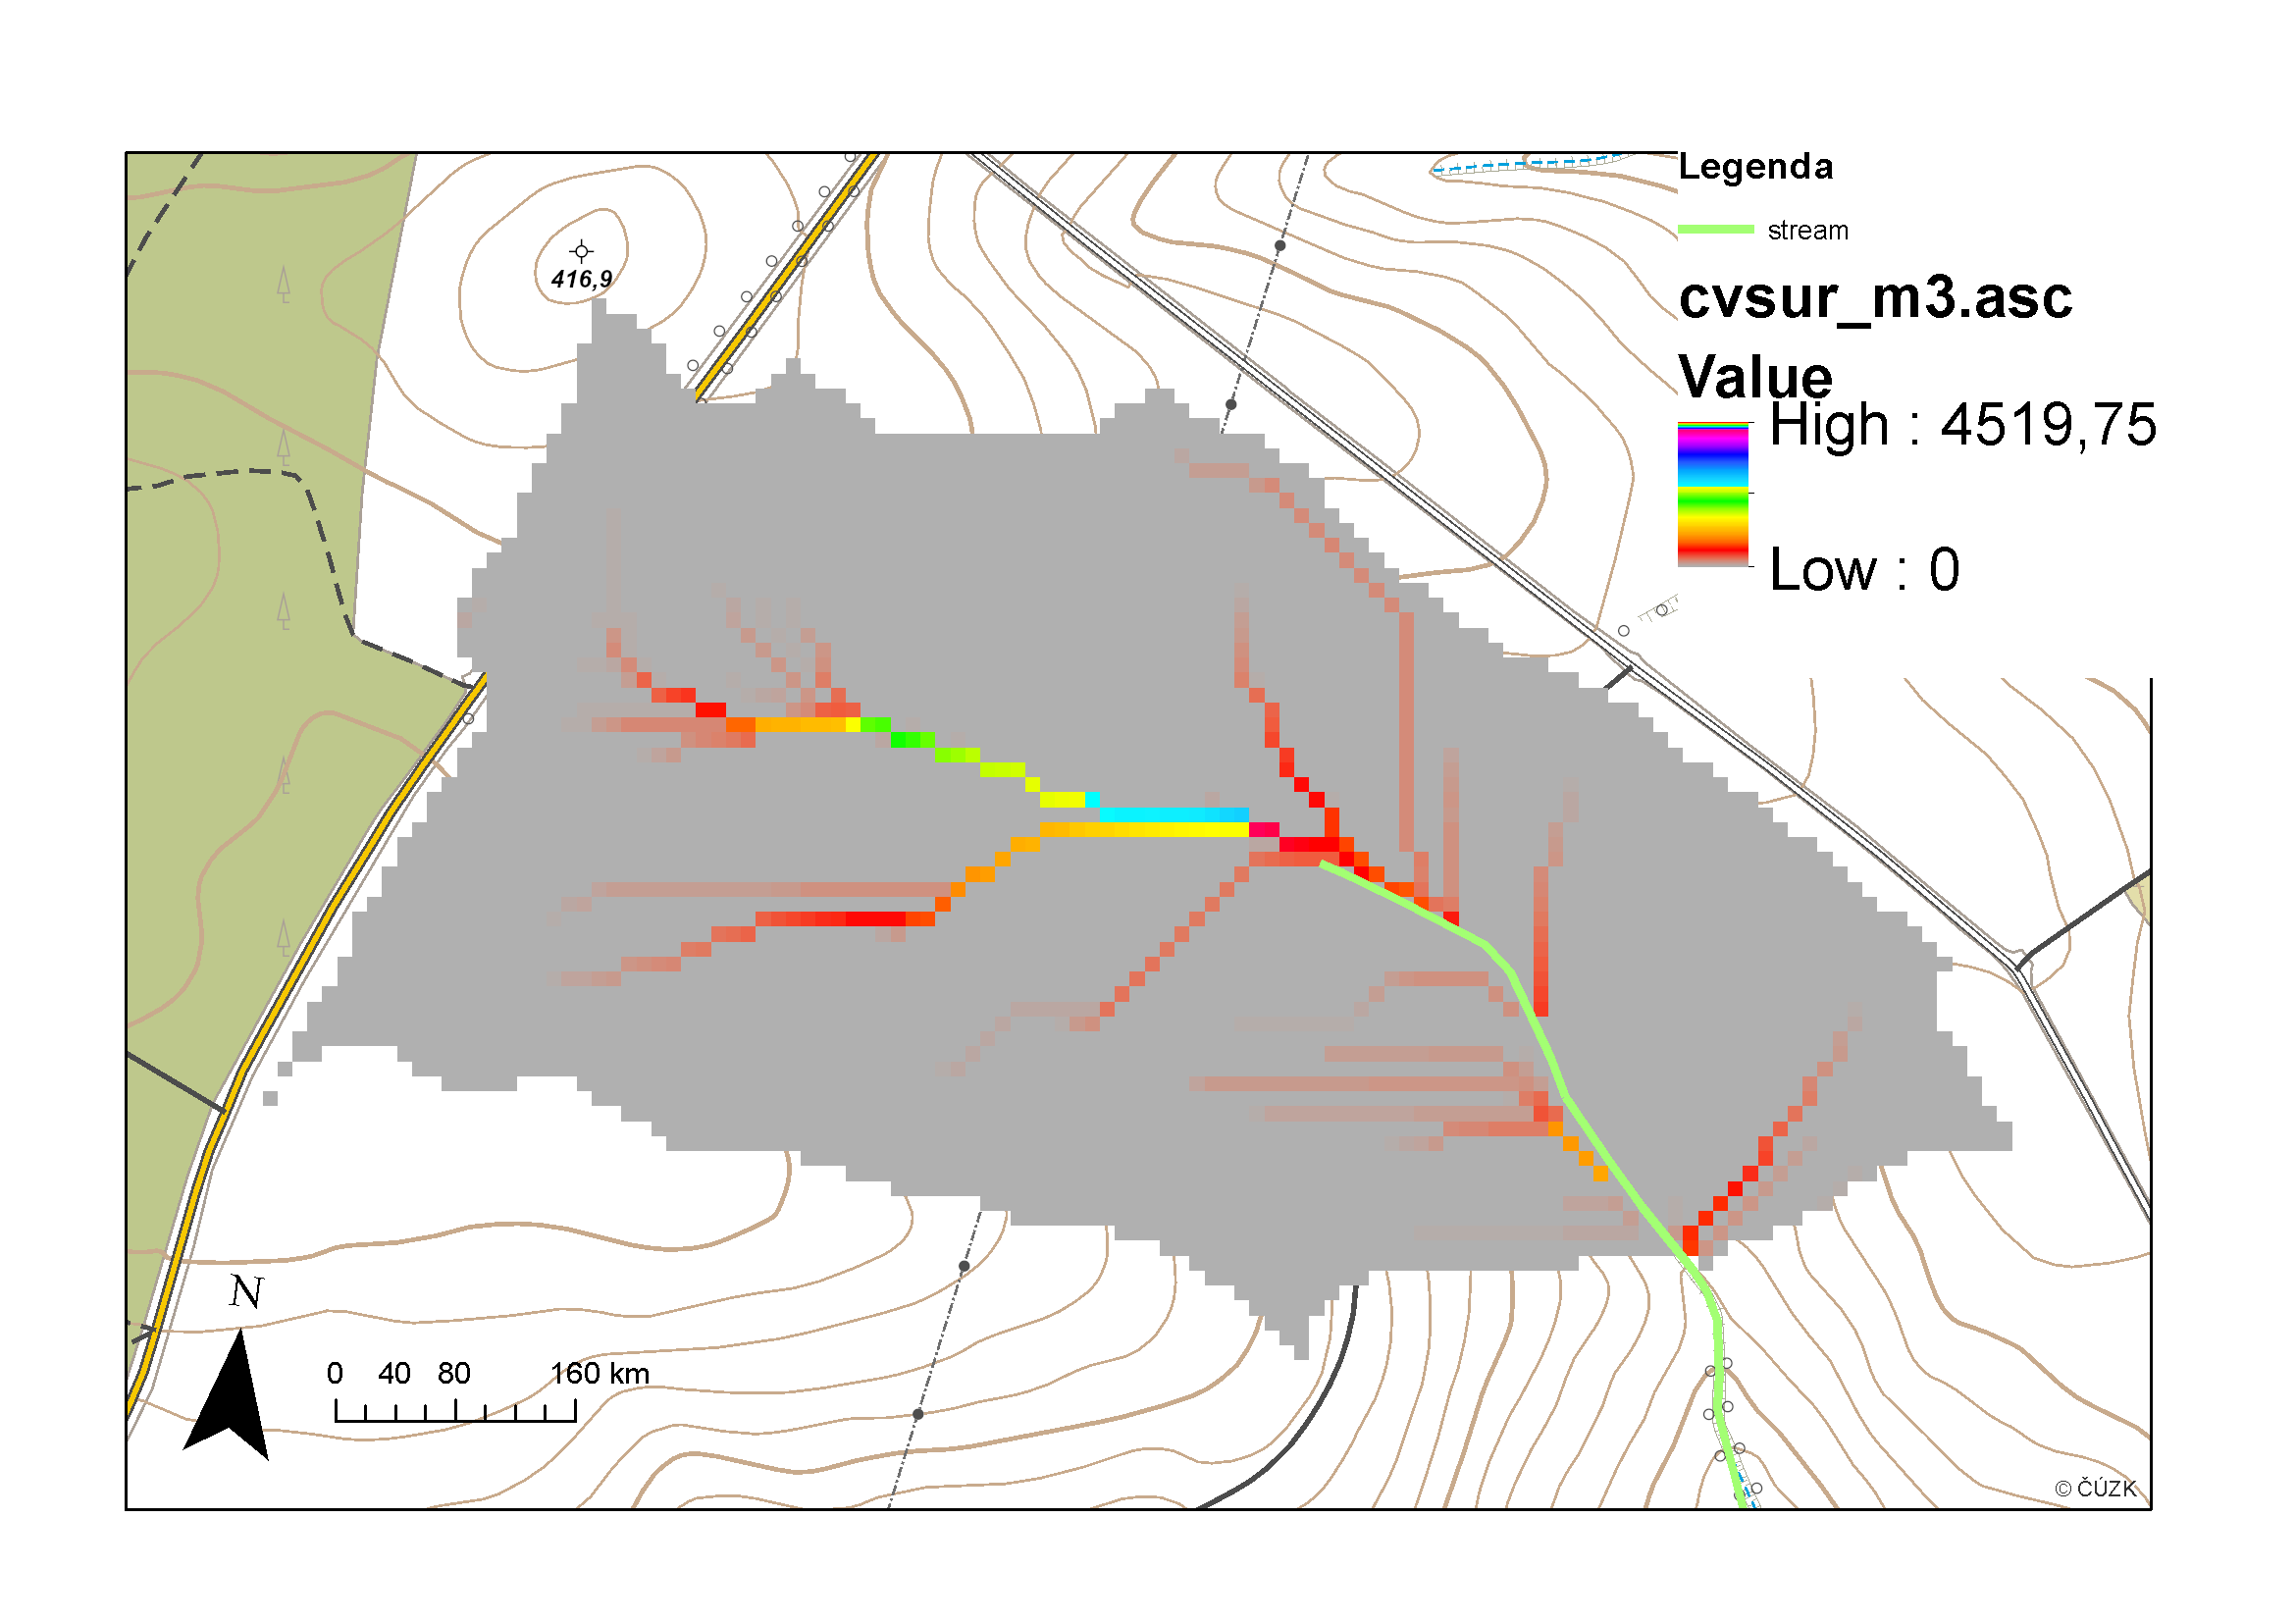
\includegraphics[width=0.55\textwidth]{obr/cvsur.png}\\
                    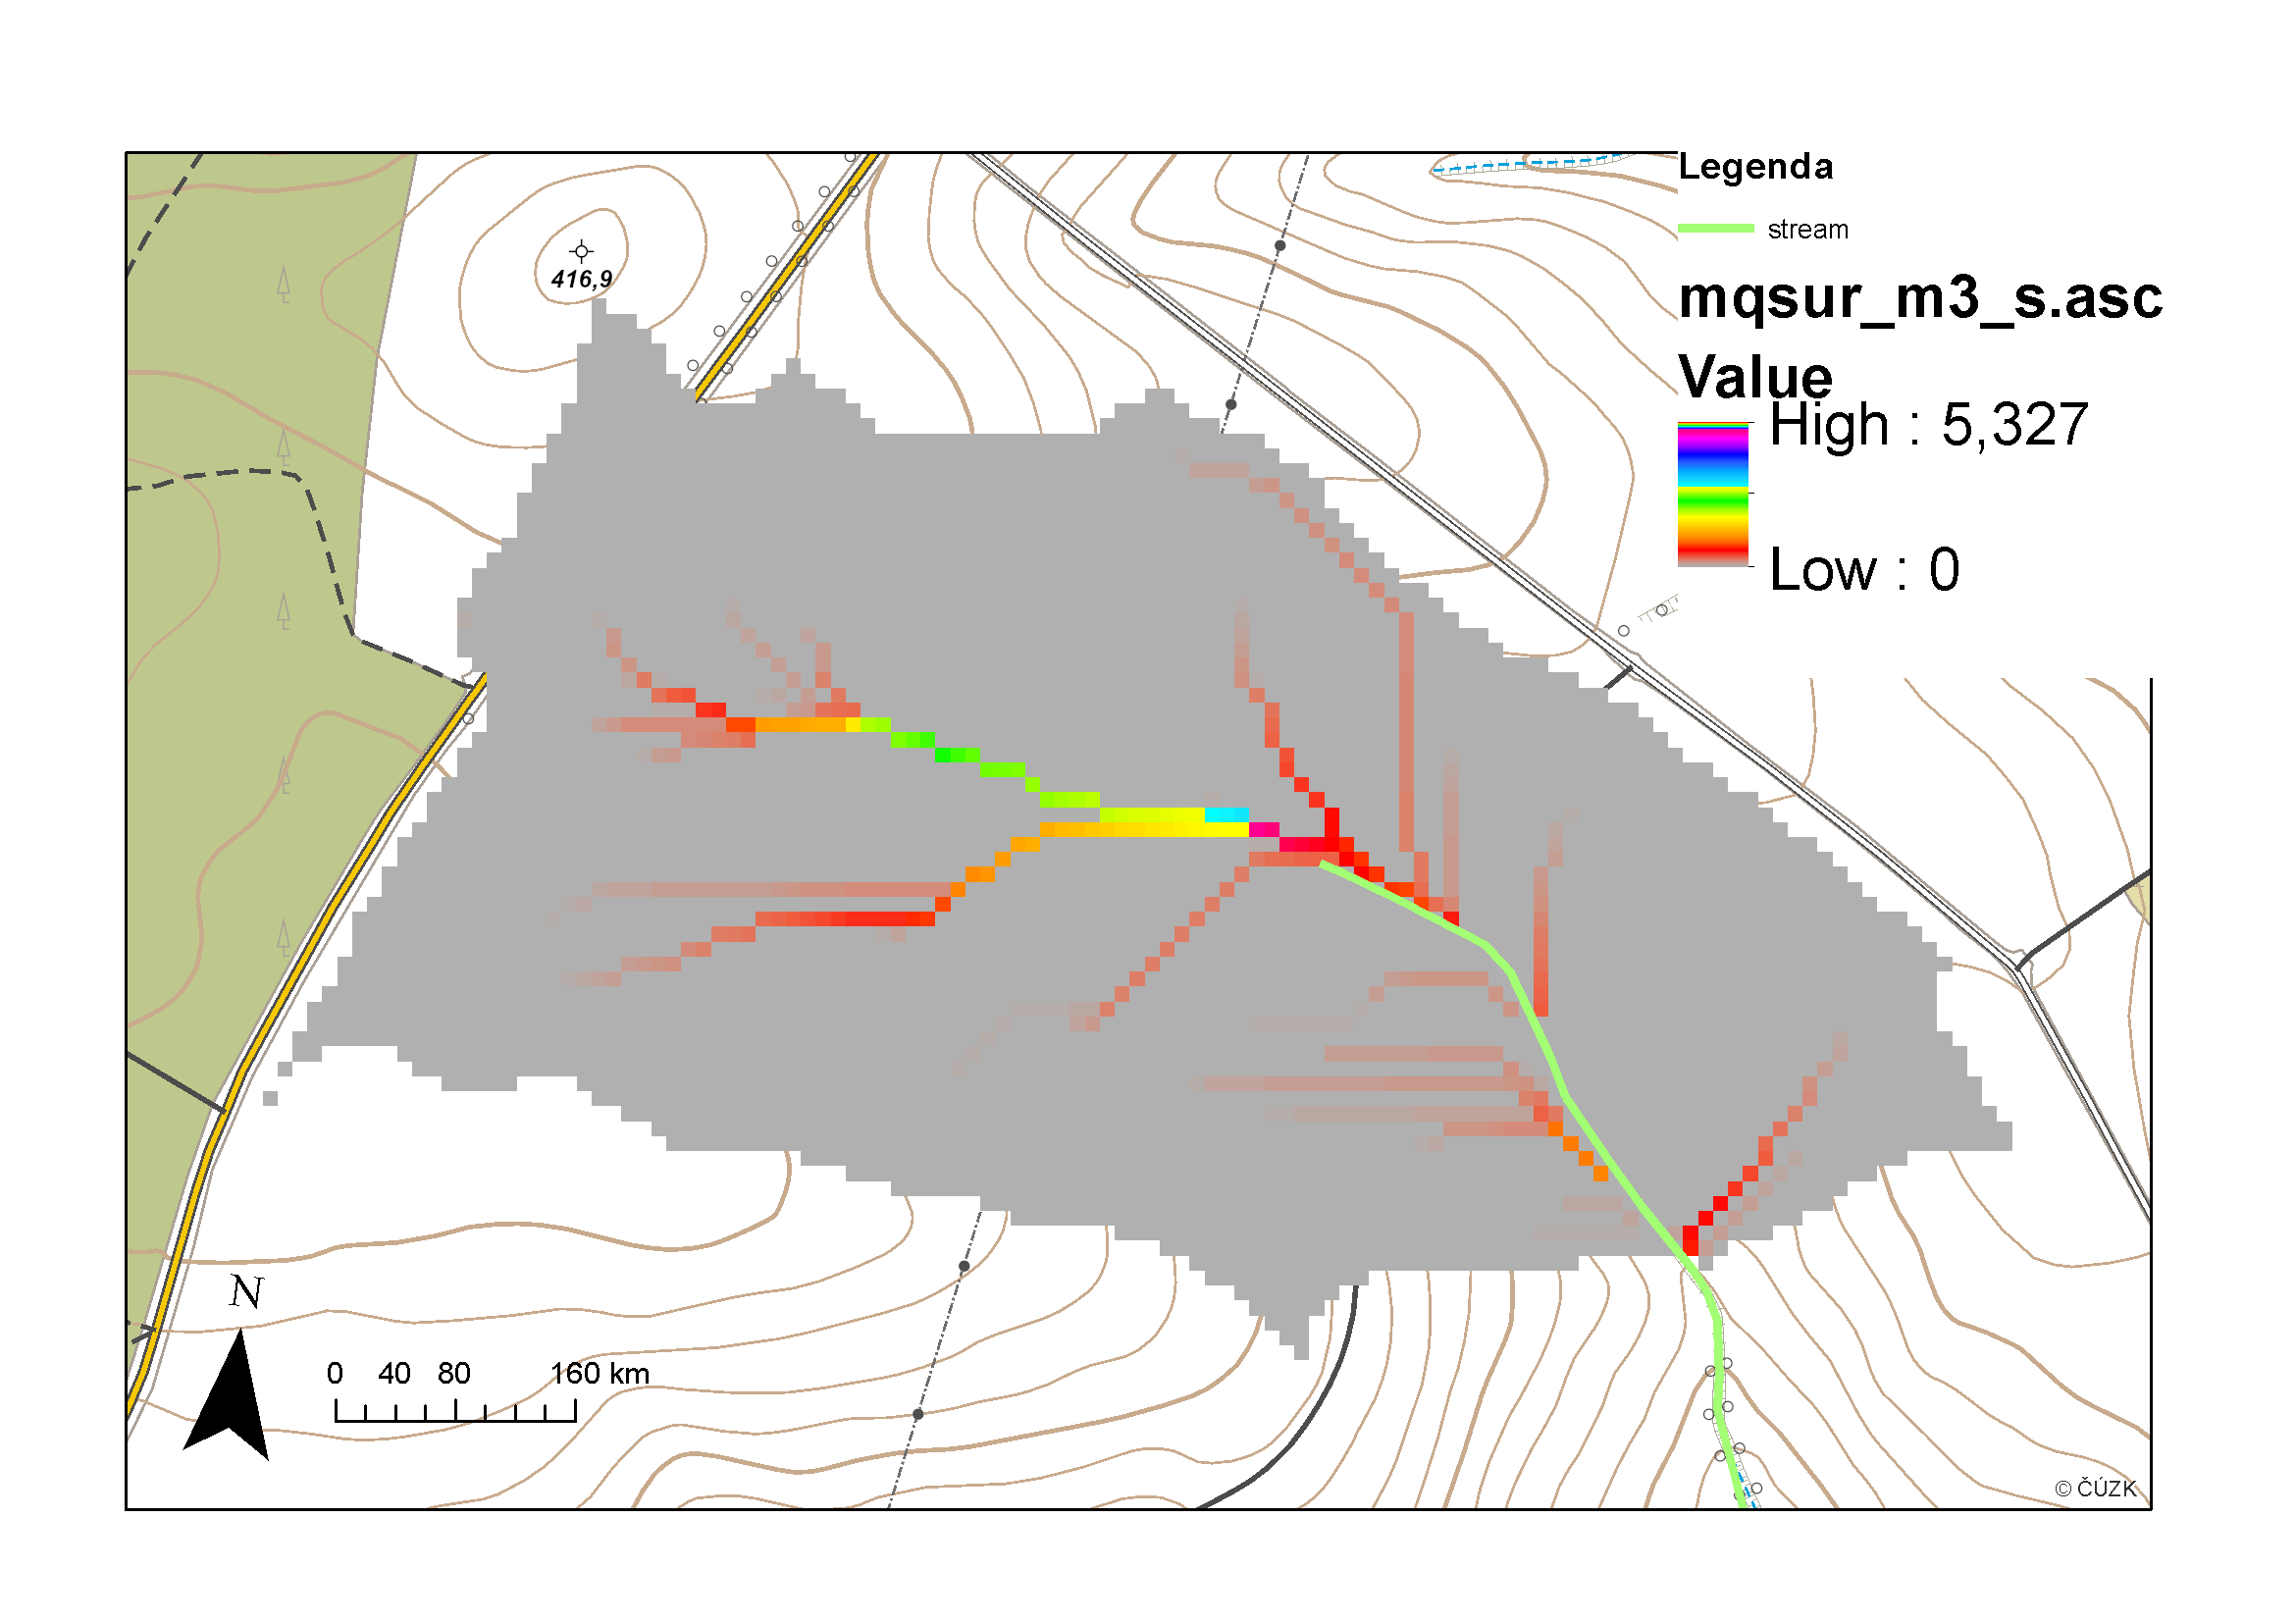
\includegraphics[width=0.55\textwidth]{obr/mqsur.png}
                    %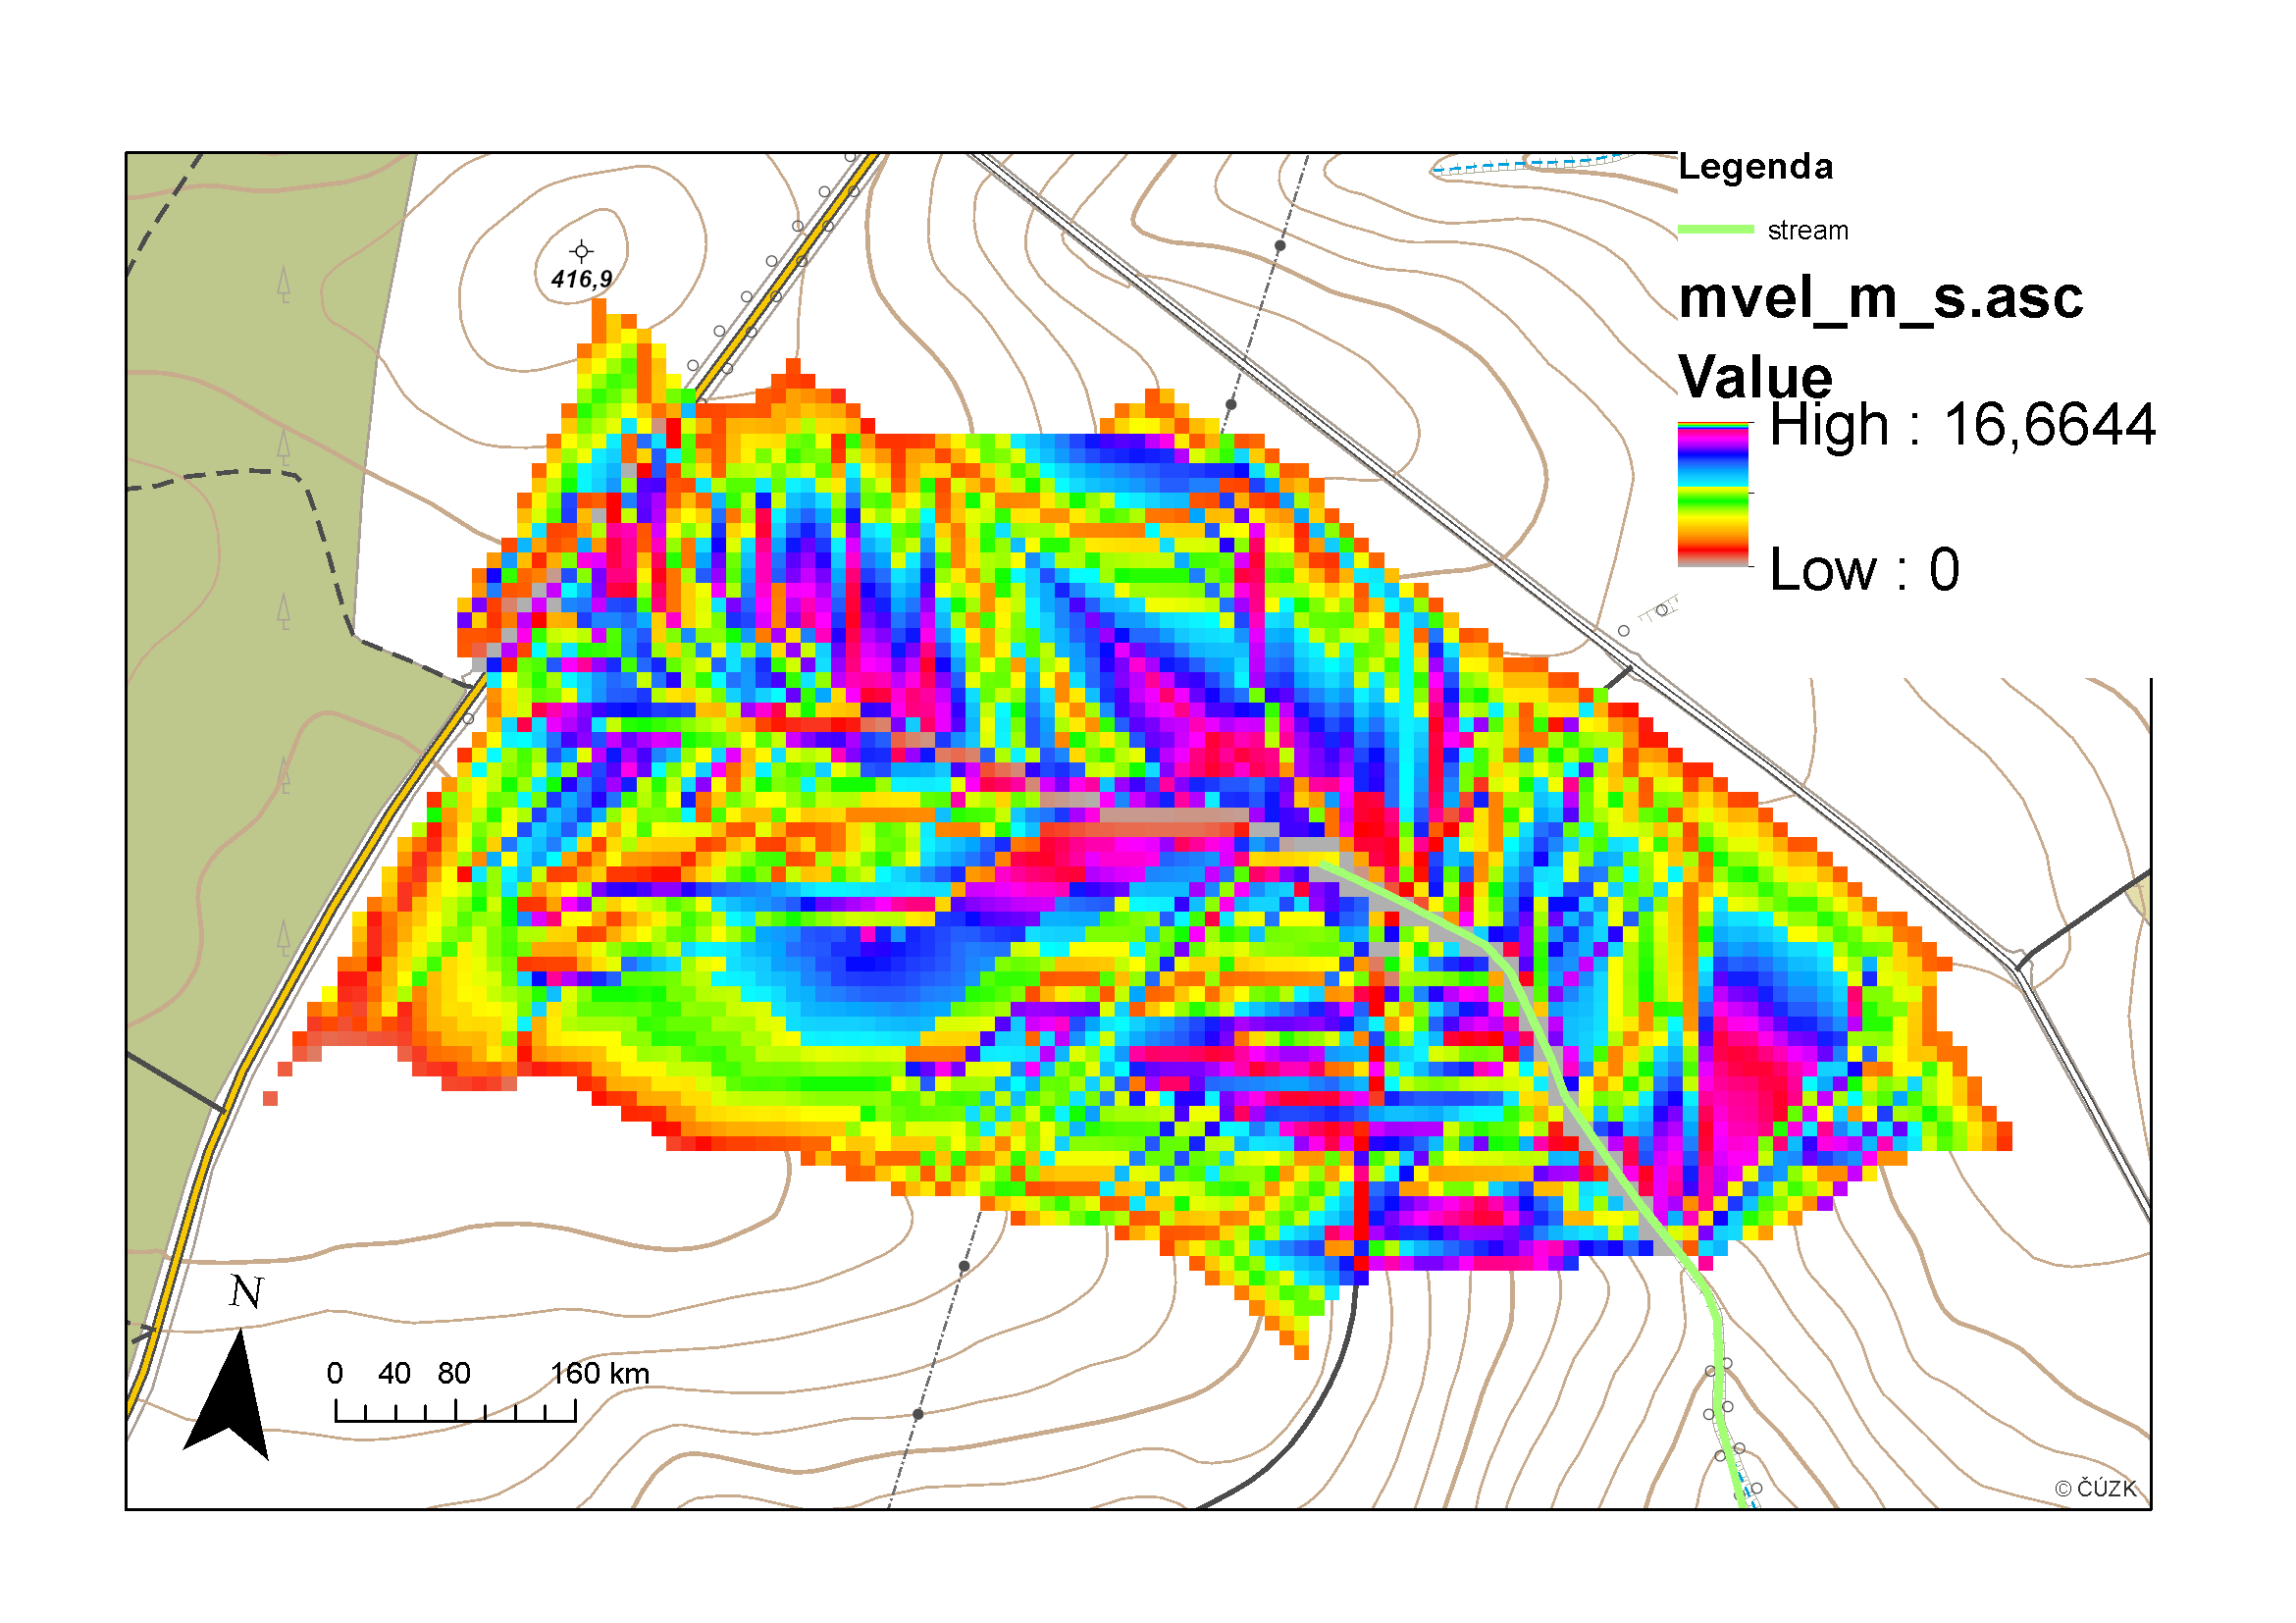
\includegraphics[width=0.55\textwidth]{obr/mvel.png}
                    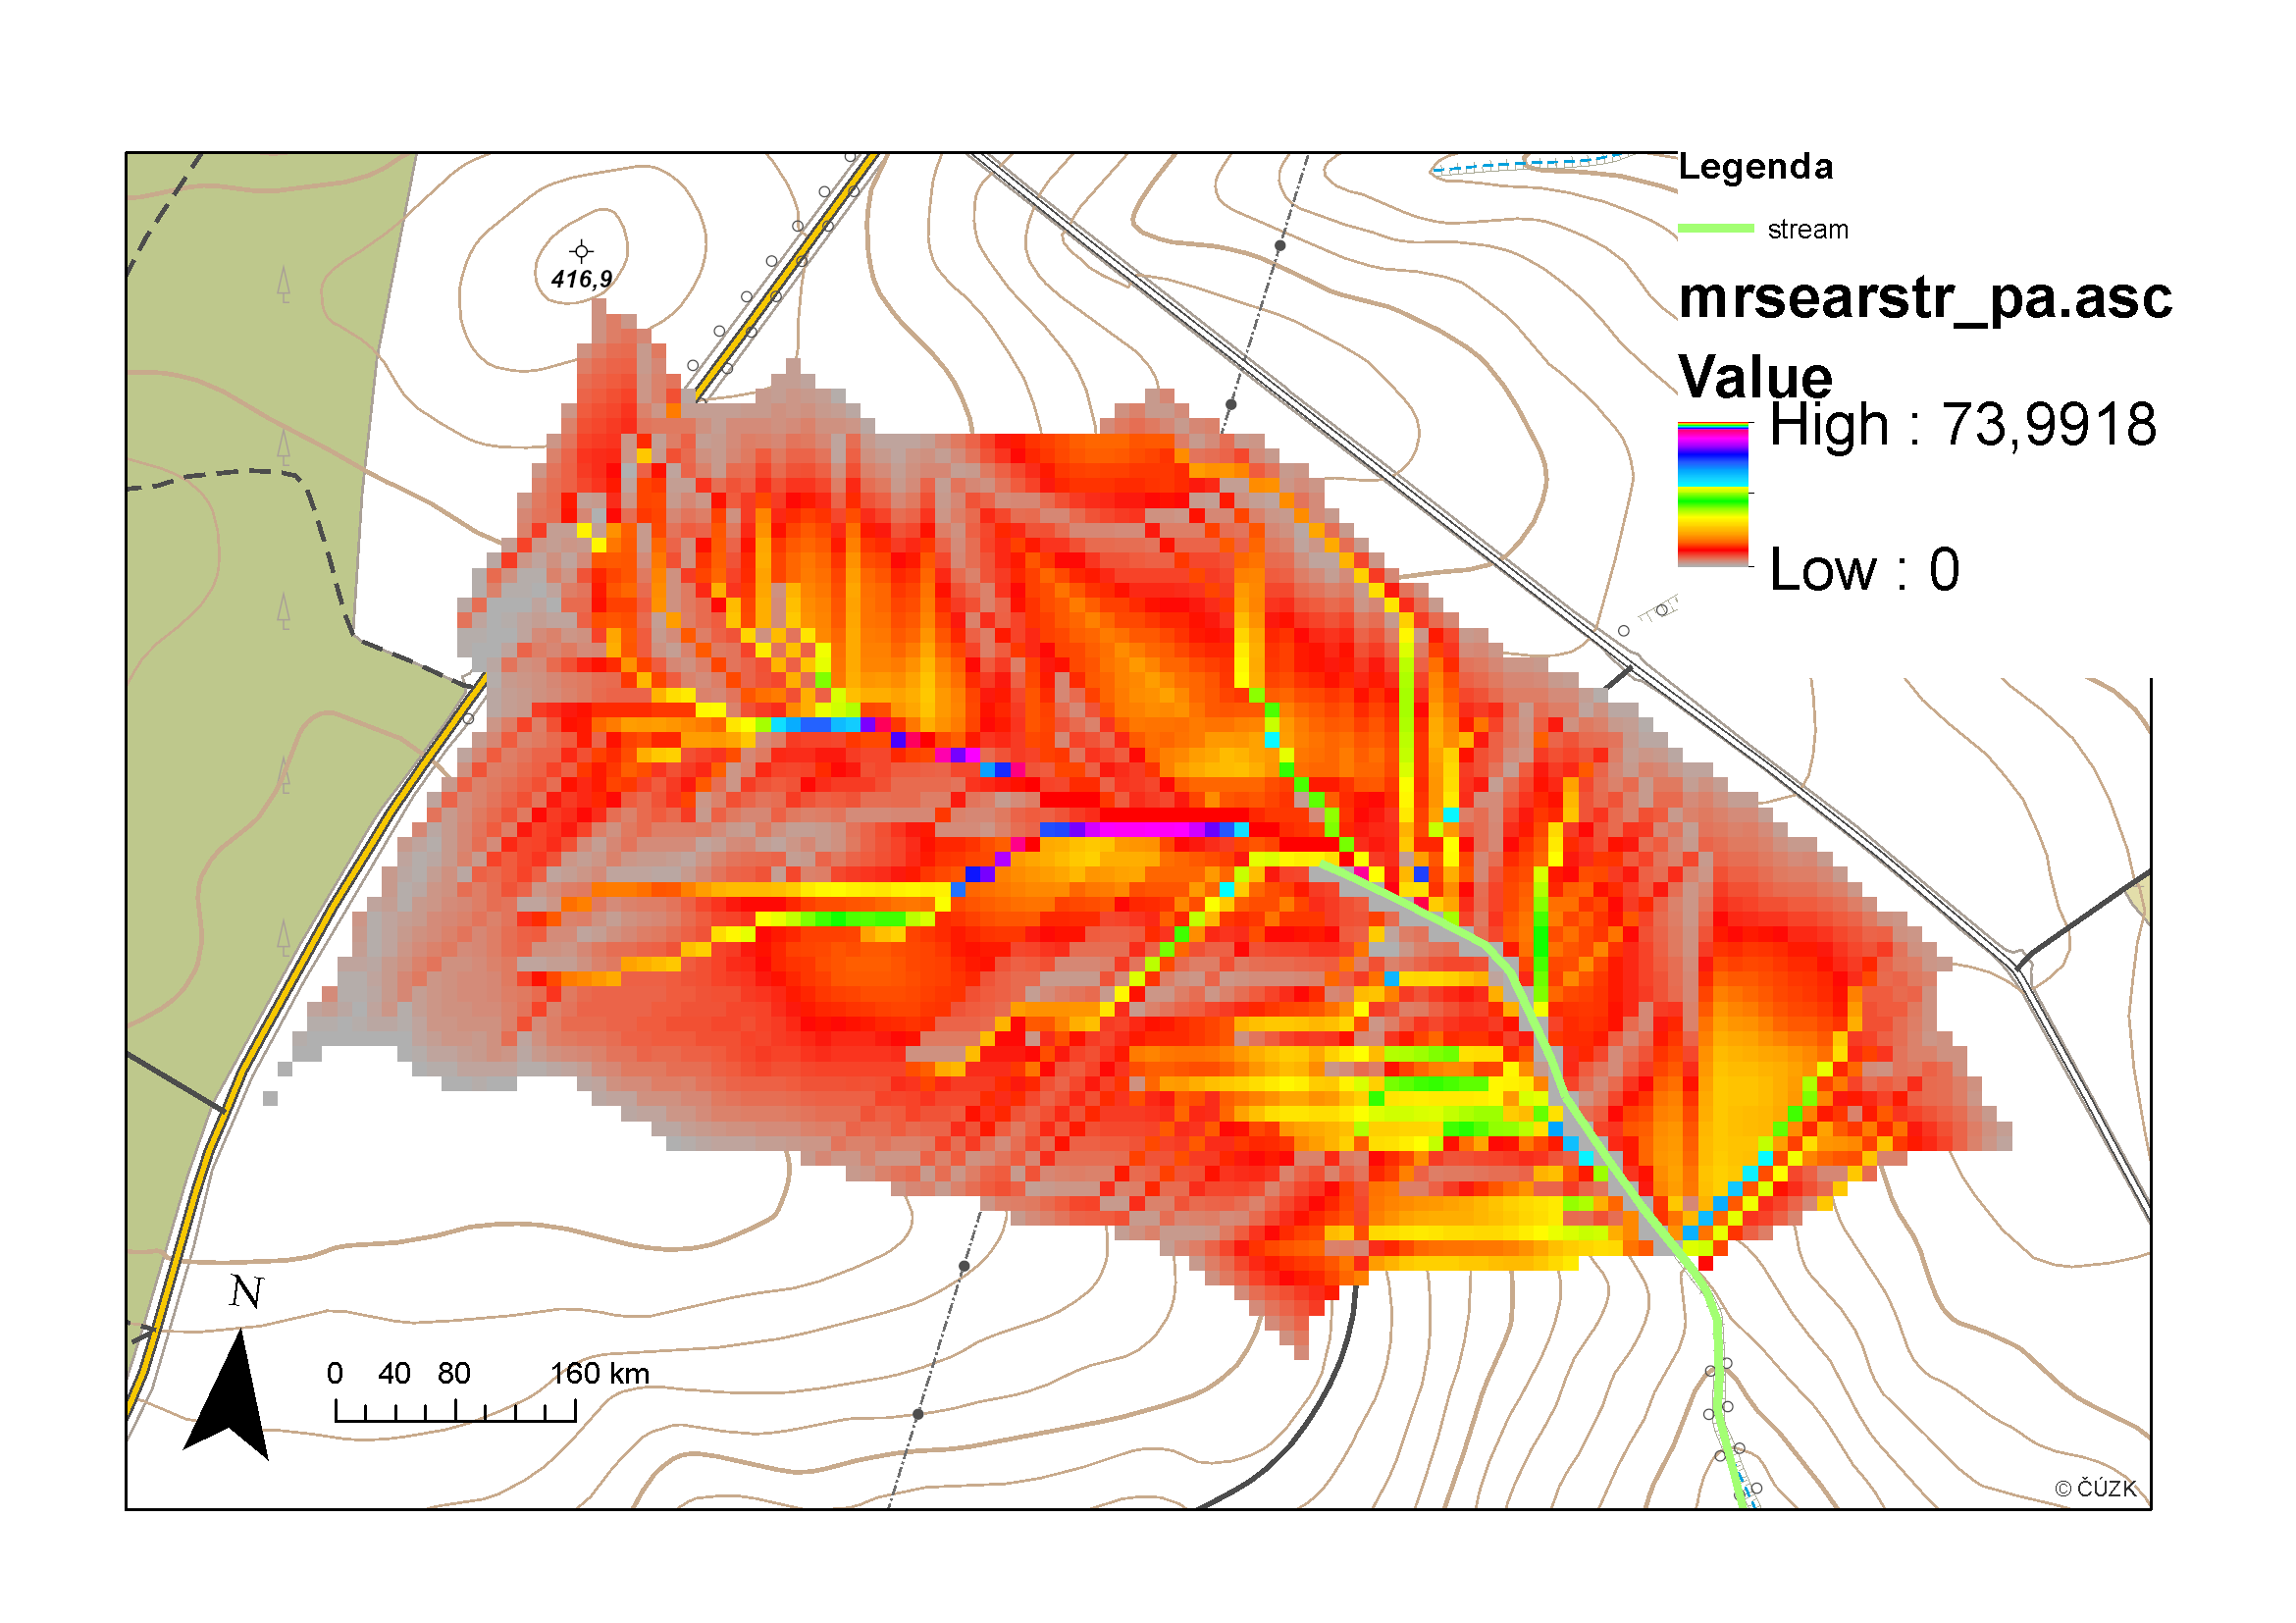
\includegraphics[width=0.55\textwidth]{obr/mshear.png}
            \end{adjustwidth}
        \end{frame}


        \begin{frame}[plain]
            Ukázka výsledků reakce povodí na 40 minut 120 mm/hod srážky
            %\begin{adjustwidth}{-4em}{-3em}
                %\begin{columns}
                    %\begin{column}{0.5\textwidth}
                    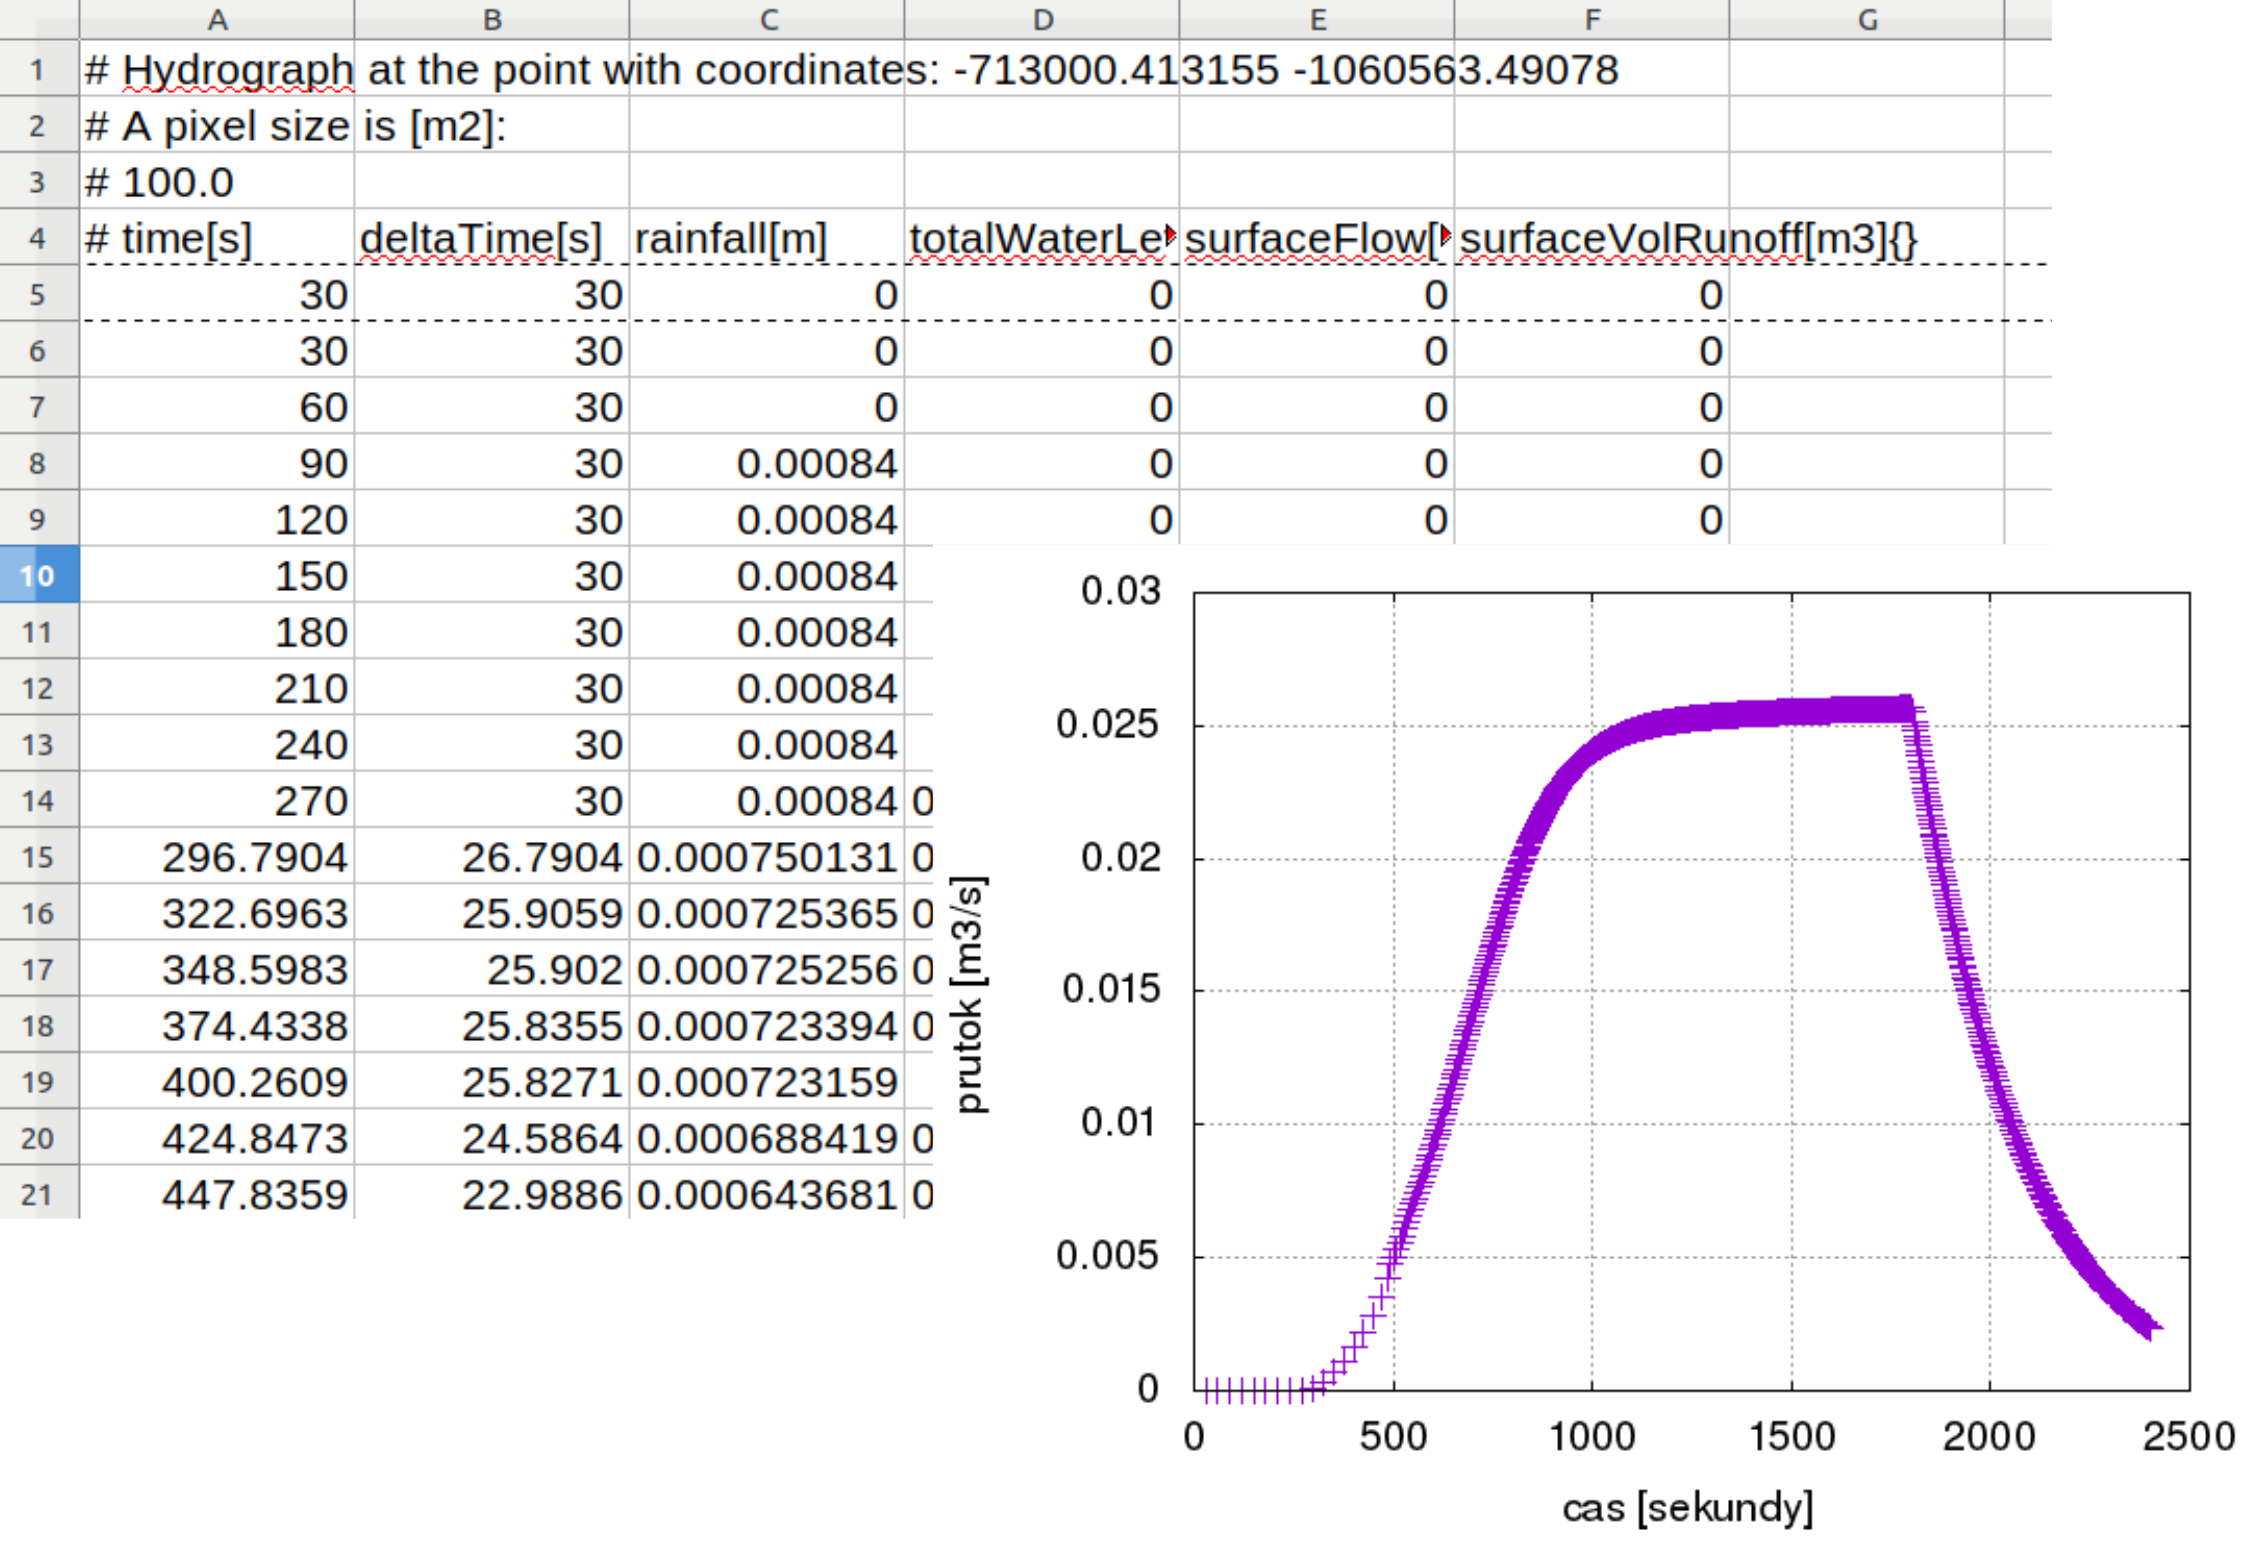
\includegraphics[width=0.9\textwidth]{obr/pointtab.png}
                    %\end{column}
                    %\begin{column}{0.5\textwidth}
                    %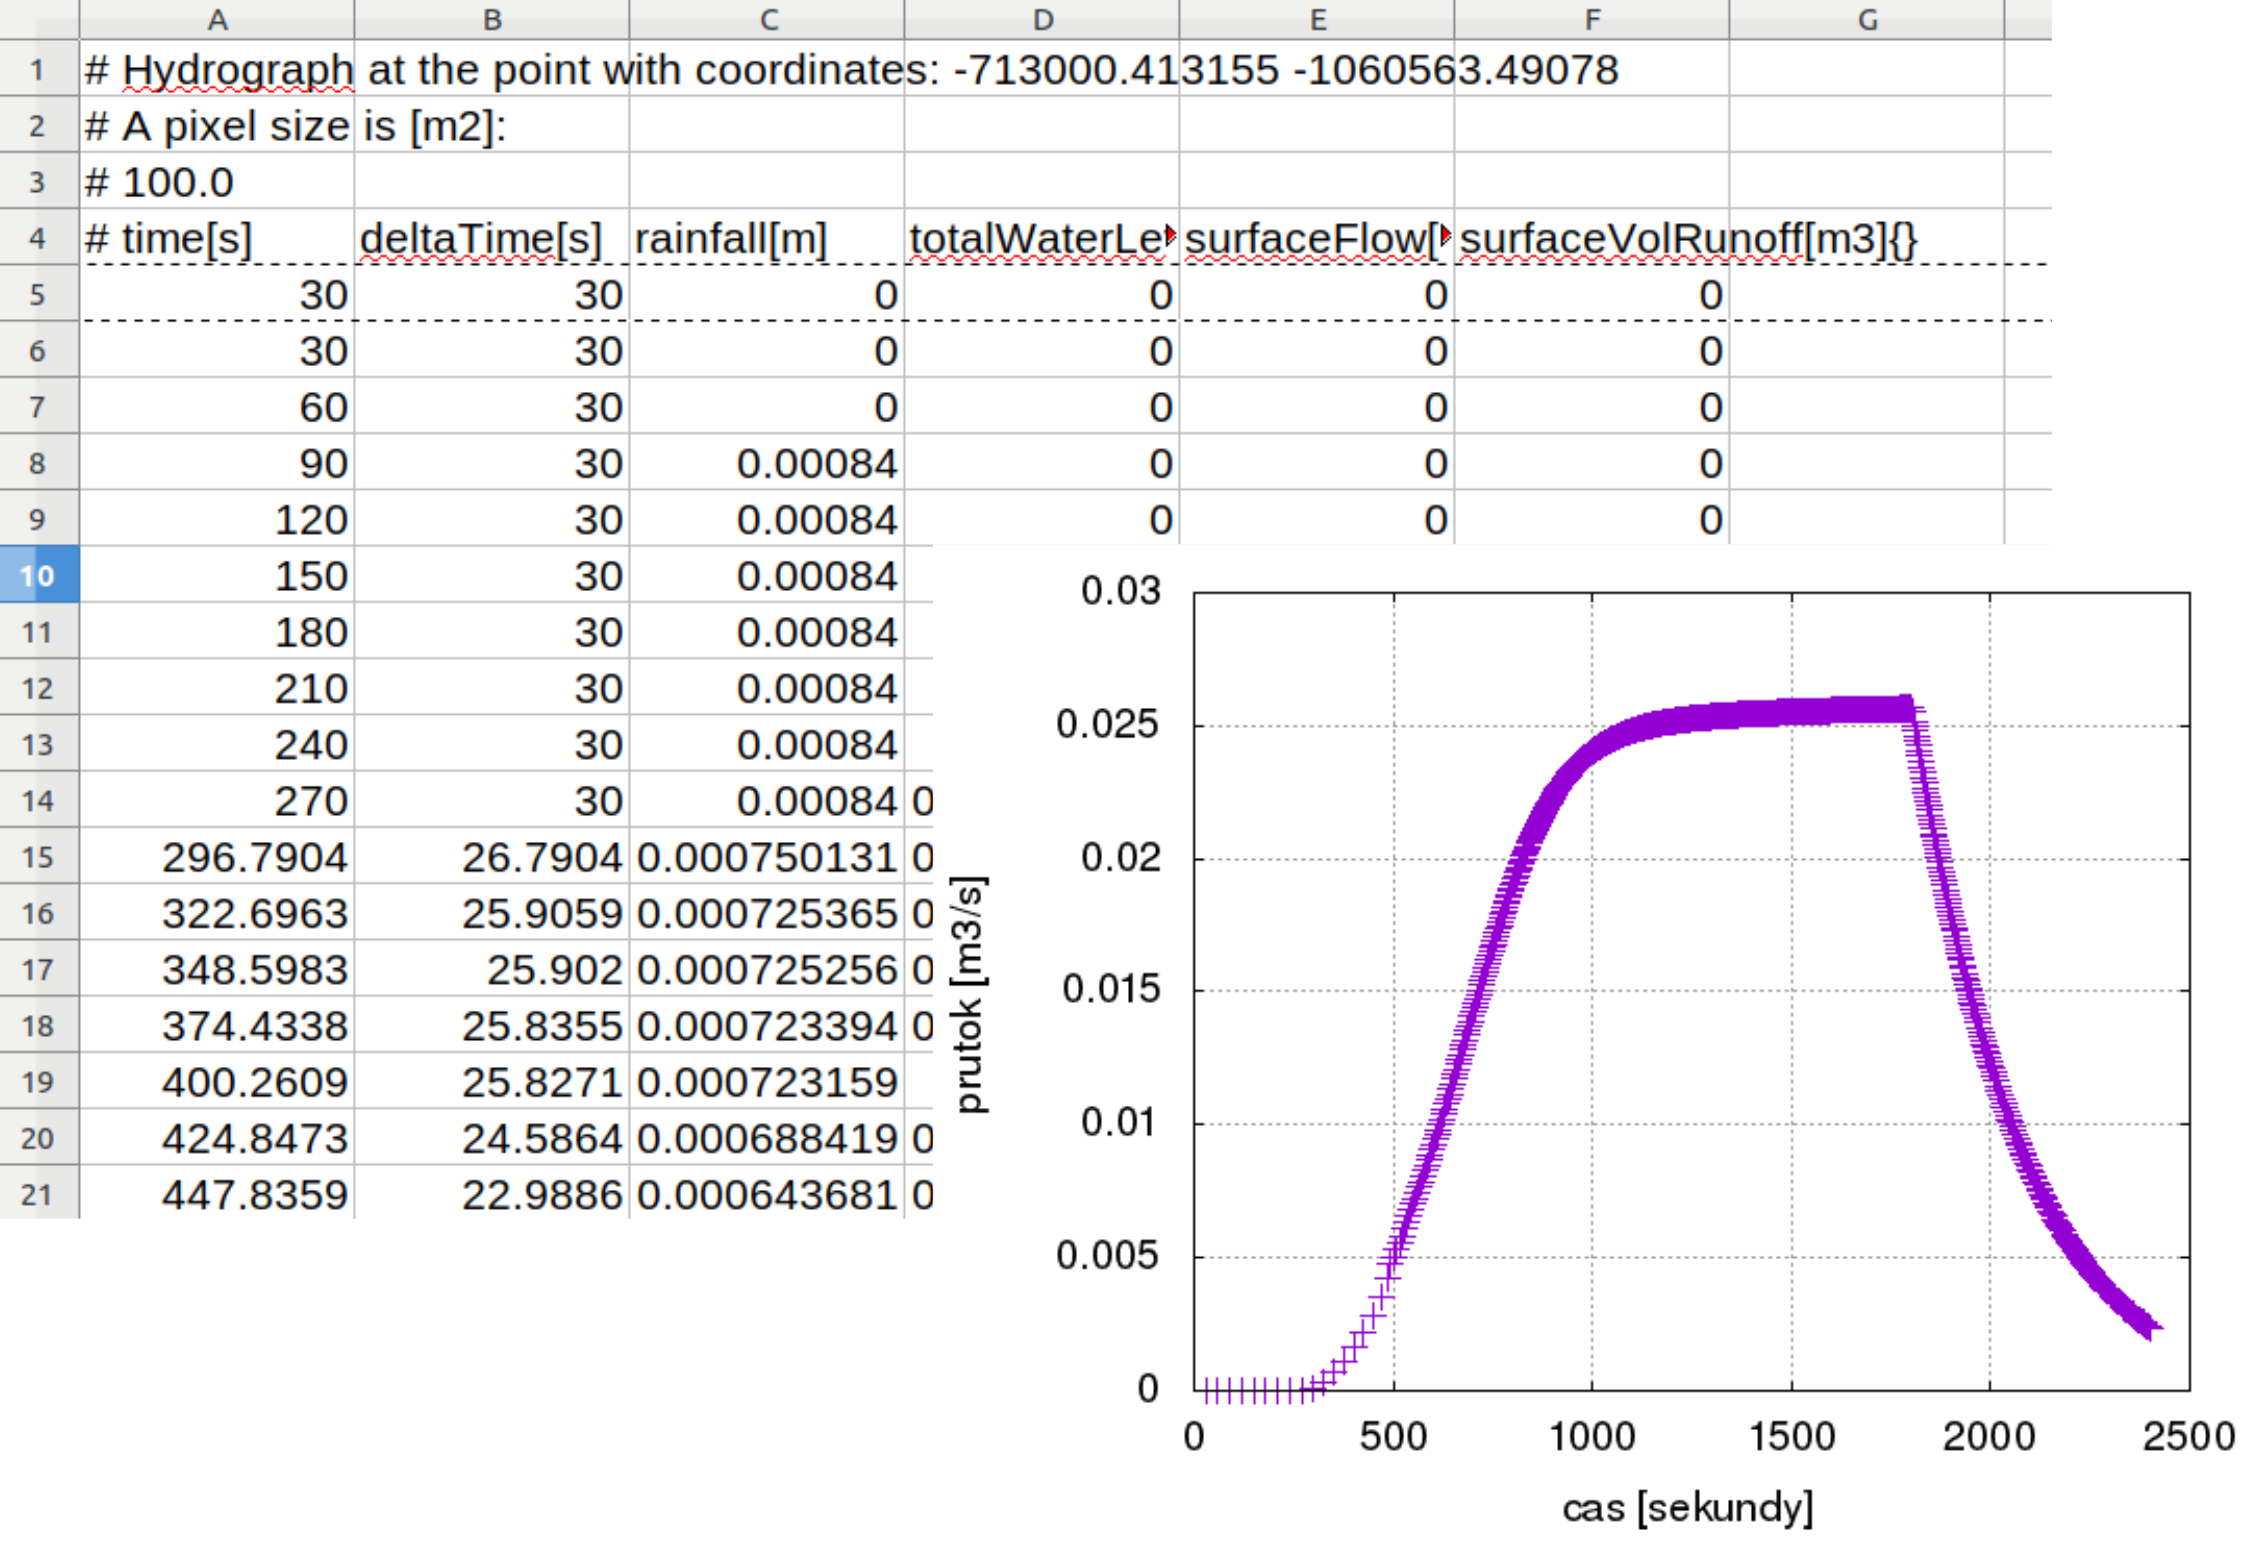
\includegraphics[width=1.1\textwidth]{obr/pointtab.png}
                    %\end{column}
                %\end{columns}
            %\end{adjustwidth}
        \end{frame}
